\documentclass[a4paper,11pt]{article}
\usepackage[margin=21mm,headheight=15pt]{geometry}
\usepackage[T1]{fontenc}
\usepackage{lmodern,amsmath,amssymb,booktabs,longtable,array}
\usepackage{tikz}
\usetikzlibrary{arrows.meta,positioning,calc,shapes.gates.logic.US}
\usepackage{xcolor,graphicx,fancyhdr,enumitem,hyperref}
\definecolor{ink}{HTML}{19354D}
\definecolor{accent}{HTML}{116B80}
\hypersetup{colorlinks=true,linkcolor=accent,urlcolor=accent,pdftitle={Lab 9: Seven-Segment Displays and Code Converters}}
\setlist{nosep,leftmargin=2em}
\setlength{\parskip}{0.4em}
\setlength{\emergencystretch}{2em}
\renewcommand{\arraystretch}{1.18}
\pagestyle{fancy}\fancyhf{}
\fancyhead[L]{\small CPE100L -- Lab 9}
\fancyhead[R]{\small Design and Analysis Report}
\fancyfoot[C]{\thepage}
\newcommand{\pending}{\textcolor{gray}{Pending}}
\newcommand{\photo}[1]{\begin{center}\fbox{\parbox[c][1.15cm][c]{0.9\linewidth}{\centering\small Photo to add: #1}}\end{center}}
\title{\textbf{Lab 9: Seven-Segment Displays\\and Code Converters}\\[0.5em]\large Complete Prelab and Postlab Derivations}
\author{Name: \underline{\hspace{3cm}}\qquad Student ID: \underline{\hspace{3cm}}}
\date{Course: CPE100L\qquad Experiment date: \underline{\hspace{2.5cm}}}
\graphicspath{{output/pdf/}{./}}
\begin{document}
\maketitle
\begin{center}\large\textcolor{accent}{Karnaugh maps -- Boolean minimization -- Circuit connections}\end{center}

\noindent\textbf{Scope of this report.} This English version contains the same design,
derivations, connection plans, expected results, and postlab answers as the Chinese version,
with exhaustive offline Boolean checks. Quartus compilation, ModelSim simulation, and
DE0-CV board testing have not been performed. Expected results are identified separately
from measurements. Design diagrams use LaTeX/TikZ; the appendix adds attributed external circuit illustrations. Board photographs, LE counts,
actual time spent, and TA sign-off remain to be supplied.

\noindent\textbf{Source and segment-pattern convention.} The task requirements come from
pages 4--7 of \texttt{CPE\_100\_Lab\_9.pdf}; the operation-select codes are confirmed by
pages 2--3 of the adjacent Lab 8 handout. On page 2 of Lab 9, the prose says that 6 omits
segment a and 9 omits segment d, but Table 2 assigns 0 to both positions, which lights them.
This report consistently follows the numeric entries in \textbf{Tables 2 and 3}: a is on
for 6, and d is on for 9. If the TA instead requires the prose convention, update the
truth table and repeat the minimization rather than mixing the two conventions.

\noindent\textbf{Experiment 3 diagram ambiguity.} The handout requests two
\texttt{hex7seg} symbols and also an independent letter decoder for HEX1. The direct
implementation here uses one \texttt{hex7seg} for the result on HEX0 and a separate
letter decoder for HEX1, because lowercase o is not a standard hexadecimal glyph.
Section~\ref{sec:lettervariant} also gives a complete alternative that retains a second
\texttt{hex7seg} and overrides its OR-mode glyph.

\clearpage\begingroup\small\setlength{\parskip}{0pt}\tableofcontents\endgroup
\clearpage
\section{Notation, segment patterns, and minimization method}
\subsection{Bit order and active-low outputs}
Define the display-decoder inputs as $D=d_3$, $C=d_2$, $B=d_1$, and $A=d_0$.
$D$ is the most significant bit and $A$ is the least significant bit. These names are
separate from the ALU operands $a_1a_0$ and $b_1b_0$.

Juxtaposition denotes AND, $+$ denotes Boolean OR, an overbar denotes NOT, and
$\oplus$ denotes XOR. Arithmetic addition is explicitly described as a sum or an ADD
operation. The segment vector is always written in the order $(a,b,c,d,e,f,g)$:
\textbf{0 turns a segment on; 1 turns it off}.


\begin{center}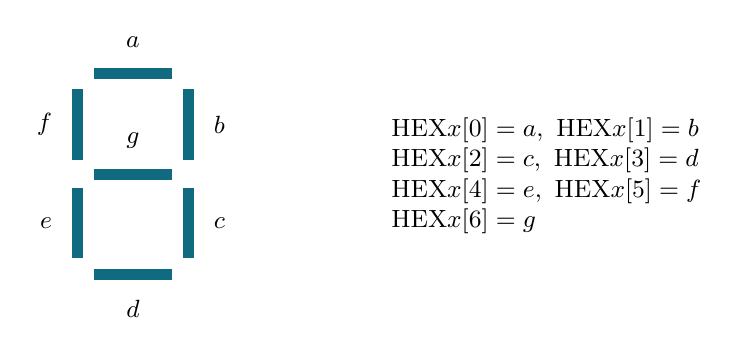
\begin{tikzpicture}[>=Latex,block/.style={draw=ink,rounded corners=2pt,fill=blue!4,minimum height=.9cm,align=center},font=\small,scale=1,transform shape]
\draw[line width=4pt,accent] (0.25,2)--(1.25,2) node[midway,above=4pt,text=black] {$a$};
\draw[line width=4pt,accent] (1.45,1.8)--(1.45,0.9) node[midway,right=4pt,text=black] {$b$};
\draw[line width=4pt,accent] (1.45,0.55)--(1.45,-0.35) node[midway,right=4pt,text=black] {$c$};
\draw[line width=4pt,accent] (0.25,-0.55)--(1.25,-0.55) node[midway,below=4pt,text=black] {$d$};
\draw[line width=4pt,accent] (0.05,0.55)--(0.05,-0.35) node[midway,left=4pt,text=black] {$e$};
\draw[line width=4pt,accent] (0.05,1.8)--(0.05,0.9) node[midway,left=4pt,text=black] {$f$};
\draw[line width=4pt,accent] (0.25,0.72)--(1.25,0.72) node[midway,above=4pt,text=black] {$g$};
\node[align=left] at (6,.7) {$\mathrm{HEX}x[0]=a,\ \mathrm{HEX}x[1]=b$\\
$\mathrm{HEX}x[2]=c,\ \mathrm{HEX}x[3]=d$\\
$\mathrm{HEX}x[4]=e,\ \mathrm{HEX}x[5]=f$\\$\mathrm{HEX}x[6]=g$};
\end{tikzpicture}\end{center}

For a bus written as $\mathrm{HEX}x[6:0]$, the left-to-right bit string is
$gfedcba$. Reverse the $abcdefg$ strings in this report when writing that bus value.
The decimal point is not used.
\subsection{Complete target truth table}
The BCD decoder constrains only inputs 0--9; inputs 10--15 are X for all seven outputs.
The hexadecimal decoder constrains all sixteen inputs and has no don't-cares.


\begin{center}\small
\begin{tabular}{rccccc}
\toprule
Value & $DCBA$ & Glyph & $abcdefg$ & $gfedcba$ & Valid BCD?\\\midrule
0 & \texttt{0000} & 0 & \texttt{0000001} & \texttt{1000000} & Yes\\
1 & \texttt{0001} & 1 & \texttt{1001111} & \texttt{1111001} & Yes\\
2 & \texttt{0010} & 2 & \texttt{0010010} & \texttt{0100100} & Yes\\
3 & \texttt{0011} & 3 & \texttt{0000110} & \texttt{0110000} & Yes\\
4 & \texttt{0100} & 4 & \texttt{1001100} & \texttt{0011001} & Yes\\
5 & \texttt{0101} & 5 & \texttt{0100100} & \texttt{0010010} & Yes\\
6 & \texttt{0110} & 6 & \texttt{0100000} & \texttt{0000010} & Yes\\
7 & \texttt{0111} & 7 & \texttt{0001111} & \texttt{1111000} & Yes\\
8 & \texttt{1000} & 8 & \texttt{0000000} & \texttt{0000000} & Yes\\
9 & \texttt{1001} & 9 & \texttt{0000100} & \texttt{0010000} & Yes\\
10 & \texttt{1010} & A & \texttt{0001000} & \texttt{0001000} & No (X)\\
11 & \texttt{1011} & b & \texttt{1100000} & \texttt{0000011} & No (X)\\
12 & \texttt{1100} & C & \texttt{0110001} & \texttt{1000110} & No (X)\\
13 & \texttt{1101} & d & \texttt{1000010} & \texttt{0100001} & No (X)\\
14 & \texttt{1110} & E & \texttt{0110000} & \texttt{0000110} & No (X)\\
15 & \texttt{1111} & F & \texttt{0111000} & \texttt{0001110} & No (X)\\
\bottomrule\end{tabular}\end{center}


\clearpage\subsection{How to read and simplify every K-map}
\begin{enumerate}
\item Rows use $DC$ and columns use $BA$, both ordered $00,01,11,10$. The small gray
number inside each cell is its minterm index $m=8D+4C+2B+A$.
\item Enter the target output values. Since the functions being minimized are the
actual active-low outputs, \textbf{group the 1s, which mean segment off}. Do not group
the illuminated 0s for the SOP functions shown here. X cells may assist a group but
do not have to be covered.
\item Form rectangular groups of 1, 2, 4, 8, or 16 cells. Groups may overlap and wrap
across opposite boundaries, but cannot contain a specified 0. Boundary pieces of the
same color belong to one group.
\item Retain variables that remain fixed within a group. A fixed 1 gives the variable;
a fixed 0 gives its complement. Eliminate changing variables. A group of $2^k$ cells
eliminates $k$ variables. For example, $\{4,5,12,13\}$ fixes $C=1,B=0$, giving
$C\overline B$.
\item OR the product terms from the groups to obtain a sum of products (SOP). The table
under each map lists every group, its covered cells, its fixed variables, and the
resulting term. This supplies the elimination steps for each output.
\end{enumerate}

Each output is minimized independently: first minimize the number of terms, then the
number of literals among solutions with that term count. The supplied checker
independently enumerates all $3^4=81$ cubes and solves an exact covering problem by
dynamic programming. Sharing is then applied by reusing identical terms in the selected
SOPs. This is \textbf{not a claim of globally optimal multi-output logic}. Two-input gate
decomposition, fan-out, and FPGA LUT mapping use different cost models.

\clearpage\section{Prelab 1: BCD-to-seven-segment decoder}
For all seven functions, the don't-care set is
$\mathcal D=\{10,11,12,13,14,15\}$. The following maps show the full minimization.


\noindent\begin{minipage}{\textwidth}

\subsection*{BCD: output $a$}

\noindent $a=\sum m\{1,4\}$; $\mathcal{D}=\{10,11,12,13,14,15\}$.

\begin{center}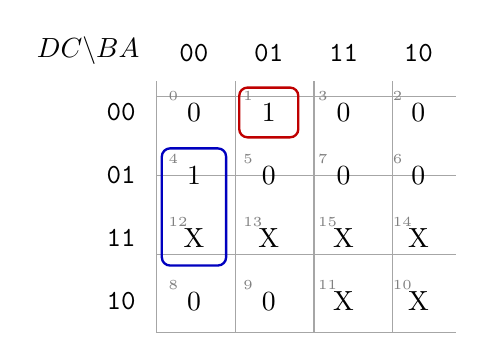
\begin{tikzpicture}[x=0.95cm,y=0.8cm,font=\normalsize]
\draw[gray!70] (0,0) grid (4,4);
\node[anchor=east] at (-0.1,4.48) {$DC\backslash BA$};
\node at (0.5,4.45) {\texttt{00}};
\node[anchor=east] at (-.15,3.5) {\texttt{00}};
\node at (1.5,4.45) {\texttt{01}};
\node[anchor=east] at (-.15,2.5) {\texttt{01}};
\node at (2.5,4.45) {\texttt{11}};
\node[anchor=east] at (-.15,1.5) {\texttt{11}};
\node at (3.5,4.45) {\texttt{10}};
\node[anchor=east] at (-.15,0.5) {\texttt{10}};
\node at (0.5,3.5) {0};
\node[font=\tiny,text=gray,anchor=north west] at (0.03,3.98) {0};
\node at (1.5,3.5) {1};
\node[font=\tiny,text=gray,anchor=north west] at (1.03,3.98) {1};
\node at (2.5,3.5) {0};
\node[font=\tiny,text=gray,anchor=north west] at (2.03,3.98) {3};
\node at (3.5,3.5) {0};
\node[font=\tiny,text=gray,anchor=north west] at (3.03,3.98) {2};
\node at (0.5,2.5) {1};
\node[font=\tiny,text=gray,anchor=north west] at (0.03,2.98) {4};
\node at (1.5,2.5) {0};
\node[font=\tiny,text=gray,anchor=north west] at (1.03,2.98) {5};
\node at (2.5,2.5) {0};
\node[font=\tiny,text=gray,anchor=north west] at (2.03,2.98) {7};
\node at (3.5,2.5) {0};
\node[font=\tiny,text=gray,anchor=north west] at (3.03,2.98) {6};
\node at (0.5,1.5) {X};
\node[font=\tiny,text=gray,anchor=north west] at (0.03,1.98) {12};
\node at (1.5,1.5) {X};
\node[font=\tiny,text=gray,anchor=north west] at (1.03,1.98) {13};
\node at (2.5,1.5) {X};
\node[font=\tiny,text=gray,anchor=north west] at (2.03,1.98) {15};
\node at (3.5,1.5) {X};
\node[font=\tiny,text=gray,anchor=north west] at (3.03,1.98) {14};
\node at (0.5,0.5) {0};
\node[font=\tiny,text=gray,anchor=north west] at (0.03,0.98) {8};
\node at (1.5,0.5) {0};
\node[font=\tiny,text=gray,anchor=north west] at (1.03,0.98) {9};
\node at (2.5,0.5) {X};
\node[font=\tiny,text=gray,anchor=north west] at (2.03,0.98) {11};
\node at (3.5,0.5) {X};
\node[font=\tiny,text=gray,anchor=north west] at (3.03,0.98) {10};
\draw[blue!75!black,line width=.85pt,rounded corners=3pt] (0.07,1.07) rectangle (0.9299999999999999,2.93);
\draw[red!75!black,line width=.85pt,rounded corners=3pt] (1.105,3.105) rectangle (1.895,3.895);
\end{tikzpicture}\end{center}

\begin{center}\small
\begin{tabular}{clll}
\toprule
Group & Cells covered (incl. X) & Fixed variables & Product term\\\midrule
\textcolor{blue!75!black}{$G_{1}$} & $\{4,12\}$ & $C=1,B=0,A=0$ & $C\overline{B}\overline{A}$\\
\textcolor{red!75!black}{$G_{2}$} & $\{1\}$ & $D=0,C=0,B=0,A=1$ & $\overline{D}\overline{C}\overline{B}A$\\
\bottomrule\end{tabular}\end{center}


\noindent OR the group terms: $\boxed{a=C\overline{B}\overline{A} + \overline{D}\overline{C}\overline{B}A}$.

\noindent Cost: 2 product term(s), 7 literal(s).

\end{minipage}\par\vspace{0.25cm}

\noindent\begin{minipage}{\textwidth}

\subsection*{BCD: output $b$}

\noindent $b=\sum m\{5,6\}$; $\mathcal{D}=\{10,11,12,13,14,15\}$.

\begin{center}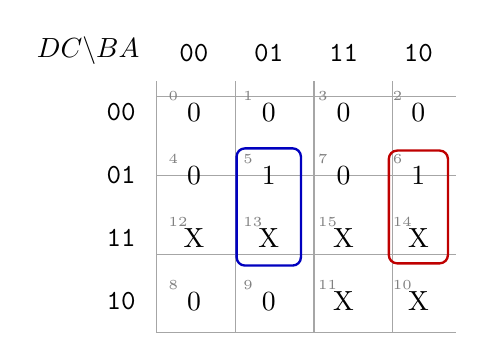
\begin{tikzpicture}[x=0.95cm,y=0.8cm,font=\normalsize]
\draw[gray!70] (0,0) grid (4,4);
\node[anchor=east] at (-0.1,4.48) {$DC\backslash BA$};
\node at (0.5,4.45) {\texttt{00}};
\node[anchor=east] at (-.15,3.5) {\texttt{00}};
\node at (1.5,4.45) {\texttt{01}};
\node[anchor=east] at (-.15,2.5) {\texttt{01}};
\node at (2.5,4.45) {\texttt{11}};
\node[anchor=east] at (-.15,1.5) {\texttt{11}};
\node at (3.5,4.45) {\texttt{10}};
\node[anchor=east] at (-.15,0.5) {\texttt{10}};
\node at (0.5,3.5) {0};
\node[font=\tiny,text=gray,anchor=north west] at (0.03,3.98) {0};
\node at (1.5,3.5) {0};
\node[font=\tiny,text=gray,anchor=north west] at (1.03,3.98) {1};
\node at (2.5,3.5) {0};
\node[font=\tiny,text=gray,anchor=north west] at (2.03,3.98) {3};
\node at (3.5,3.5) {0};
\node[font=\tiny,text=gray,anchor=north west] at (3.03,3.98) {2};
\node at (0.5,2.5) {0};
\node[font=\tiny,text=gray,anchor=north west] at (0.03,2.98) {4};
\node at (1.5,2.5) {1};
\node[font=\tiny,text=gray,anchor=north west] at (1.03,2.98) {5};
\node at (2.5,2.5) {0};
\node[font=\tiny,text=gray,anchor=north west] at (2.03,2.98) {7};
\node at (3.5,2.5) {1};
\node[font=\tiny,text=gray,anchor=north west] at (3.03,2.98) {6};
\node at (0.5,1.5) {X};
\node[font=\tiny,text=gray,anchor=north west] at (0.03,1.98) {12};
\node at (1.5,1.5) {X};
\node[font=\tiny,text=gray,anchor=north west] at (1.03,1.98) {13};
\node at (2.5,1.5) {X};
\node[font=\tiny,text=gray,anchor=north west] at (2.03,1.98) {15};
\node at (3.5,1.5) {X};
\node[font=\tiny,text=gray,anchor=north west] at (3.03,1.98) {14};
\node at (0.5,0.5) {0};
\node[font=\tiny,text=gray,anchor=north west] at (0.03,0.98) {8};
\node at (1.5,0.5) {0};
\node[font=\tiny,text=gray,anchor=north west] at (1.03,0.98) {9};
\node at (2.5,0.5) {X};
\node[font=\tiny,text=gray,anchor=north west] at (2.03,0.98) {11};
\node at (3.5,0.5) {X};
\node[font=\tiny,text=gray,anchor=north west] at (3.03,0.98) {10};
\draw[blue!75!black,line width=.85pt,rounded corners=3pt] (1.07,1.07) rectangle (1.93,2.93);
\draw[red!75!black,line width=.85pt,rounded corners=3pt] (3.105,1.105) rectangle (3.895,2.895);
\end{tikzpicture}\end{center}

\begin{center}\small
\begin{tabular}{clll}
\toprule
Group & Cells covered (incl. X) & Fixed variables & Product term\\\midrule
\textcolor{blue!75!black}{$G_{1}$} & $\{5,13\}$ & $C=1,B=0,A=1$ & $C\overline{B}A$\\
\textcolor{red!75!black}{$G_{2}$} & $\{6,14\}$ & $C=1,B=1,A=0$ & $CB\overline{A}$\\
\bottomrule\end{tabular}\end{center}


\noindent OR the group terms: $\boxed{b=C\overline{B}A + CB\overline{A}}$.

\noindent Cost: 2 product term(s), 6 literal(s).

\end{minipage}\par\vspace{0.25cm}

\clearpage

\noindent\begin{minipage}{\textwidth}

\subsection*{BCD: output $c$}

\noindent $c=\sum m\{2\}$; $\mathcal{D}=\{10,11,12,13,14,15\}$.

\begin{center}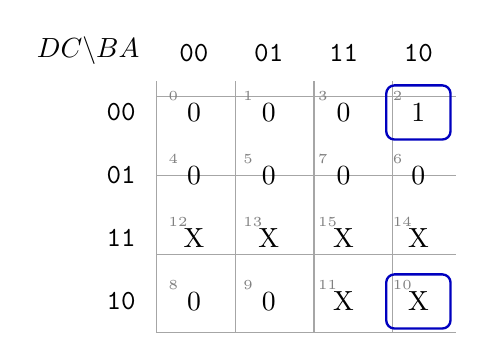
\begin{tikzpicture}[x=0.95cm,y=0.8cm,font=\normalsize]
\draw[gray!70] (0,0) grid (4,4);
\node[anchor=east] at (-0.1,4.48) {$DC\backslash BA$};
\node at (0.5,4.45) {\texttt{00}};
\node[anchor=east] at (-.15,3.5) {\texttt{00}};
\node at (1.5,4.45) {\texttt{01}};
\node[anchor=east] at (-.15,2.5) {\texttt{01}};
\node at (2.5,4.45) {\texttt{11}};
\node[anchor=east] at (-.15,1.5) {\texttt{11}};
\node at (3.5,4.45) {\texttt{10}};
\node[anchor=east] at (-.15,0.5) {\texttt{10}};
\node at (0.5,3.5) {0};
\node[font=\tiny,text=gray,anchor=north west] at (0.03,3.98) {0};
\node at (1.5,3.5) {0};
\node[font=\tiny,text=gray,anchor=north west] at (1.03,3.98) {1};
\node at (2.5,3.5) {0};
\node[font=\tiny,text=gray,anchor=north west] at (2.03,3.98) {3};
\node at (3.5,3.5) {1};
\node[font=\tiny,text=gray,anchor=north west] at (3.03,3.98) {2};
\node at (0.5,2.5) {0};
\node[font=\tiny,text=gray,anchor=north west] at (0.03,2.98) {4};
\node at (1.5,2.5) {0};
\node[font=\tiny,text=gray,anchor=north west] at (1.03,2.98) {5};
\node at (2.5,2.5) {0};
\node[font=\tiny,text=gray,anchor=north west] at (2.03,2.98) {7};
\node at (3.5,2.5) {0};
\node[font=\tiny,text=gray,anchor=north west] at (3.03,2.98) {6};
\node at (0.5,1.5) {X};
\node[font=\tiny,text=gray,anchor=north west] at (0.03,1.98) {12};
\node at (1.5,1.5) {X};
\node[font=\tiny,text=gray,anchor=north west] at (1.03,1.98) {13};
\node at (2.5,1.5) {X};
\node[font=\tiny,text=gray,anchor=north west] at (2.03,1.98) {15};
\node at (3.5,1.5) {X};
\node[font=\tiny,text=gray,anchor=north west] at (3.03,1.98) {14};
\node at (0.5,0.5) {0};
\node[font=\tiny,text=gray,anchor=north west] at (0.03,0.98) {8};
\node at (1.5,0.5) {0};
\node[font=\tiny,text=gray,anchor=north west] at (1.03,0.98) {9};
\node at (2.5,0.5) {X};
\node[font=\tiny,text=gray,anchor=north west] at (2.03,0.98) {11};
\node at (3.5,0.5) {X};
\node[font=\tiny,text=gray,anchor=north west] at (3.03,0.98) {10};
\draw[blue!75!black,line width=.85pt,rounded corners=3pt] (3.07,3.07) rectangle (3.93,3.93);
\draw[blue!75!black,line width=.85pt,rounded corners=3pt] (3.07,0.07) rectangle (3.93,0.9299999999999999);
\end{tikzpicture}\end{center}

\begin{center}\small
\begin{tabular}{clll}
\toprule
Group & Cells covered (incl. X) & Fixed variables & Product term\\\midrule
\textcolor{blue!75!black}{$G_{1}$} & $\{2,10\}$ & $C=0,B=1,A=0$ & $\overline{C}B\overline{A}$\\
\bottomrule\end{tabular}\end{center}


\noindent OR the group terms: $\boxed{c=\overline{C}B\overline{A}}$.

\noindent Cost: 1 product term(s), 3 literal(s).

\end{minipage}\par\vspace{0.25cm}

\noindent\begin{minipage}{\textwidth}

\subsection*{BCD: output $d$}

\noindent $d=\sum m\{1,4,7\}$; $\mathcal{D}=\{10,11,12,13,14,15\}$.

\begin{center}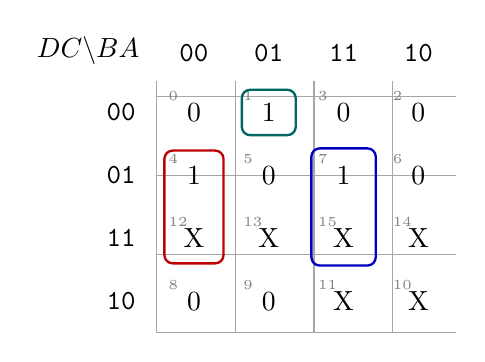
\begin{tikzpicture}[x=0.95cm,y=0.8cm,font=\normalsize]
\draw[gray!70] (0,0) grid (4,4);
\node[anchor=east] at (-0.1,4.48) {$DC\backslash BA$};
\node at (0.5,4.45) {\texttt{00}};
\node[anchor=east] at (-.15,3.5) {\texttt{00}};
\node at (1.5,4.45) {\texttt{01}};
\node[anchor=east] at (-.15,2.5) {\texttt{01}};
\node at (2.5,4.45) {\texttt{11}};
\node[anchor=east] at (-.15,1.5) {\texttt{11}};
\node at (3.5,4.45) {\texttt{10}};
\node[anchor=east] at (-.15,0.5) {\texttt{10}};
\node at (0.5,3.5) {0};
\node[font=\tiny,text=gray,anchor=north west] at (0.03,3.98) {0};
\node at (1.5,3.5) {1};
\node[font=\tiny,text=gray,anchor=north west] at (1.03,3.98) {1};
\node at (2.5,3.5) {0};
\node[font=\tiny,text=gray,anchor=north west] at (2.03,3.98) {3};
\node at (3.5,3.5) {0};
\node[font=\tiny,text=gray,anchor=north west] at (3.03,3.98) {2};
\node at (0.5,2.5) {1};
\node[font=\tiny,text=gray,anchor=north west] at (0.03,2.98) {4};
\node at (1.5,2.5) {0};
\node[font=\tiny,text=gray,anchor=north west] at (1.03,2.98) {5};
\node at (2.5,2.5) {1};
\node[font=\tiny,text=gray,anchor=north west] at (2.03,2.98) {7};
\node at (3.5,2.5) {0};
\node[font=\tiny,text=gray,anchor=north west] at (3.03,2.98) {6};
\node at (0.5,1.5) {X};
\node[font=\tiny,text=gray,anchor=north west] at (0.03,1.98) {12};
\node at (1.5,1.5) {X};
\node[font=\tiny,text=gray,anchor=north west] at (1.03,1.98) {13};
\node at (2.5,1.5) {X};
\node[font=\tiny,text=gray,anchor=north west] at (2.03,1.98) {15};
\node at (3.5,1.5) {X};
\node[font=\tiny,text=gray,anchor=north west] at (3.03,1.98) {14};
\node at (0.5,0.5) {0};
\node[font=\tiny,text=gray,anchor=north west] at (0.03,0.98) {8};
\node at (1.5,0.5) {0};
\node[font=\tiny,text=gray,anchor=north west] at (1.03,0.98) {9};
\node at (2.5,0.5) {X};
\node[font=\tiny,text=gray,anchor=north west] at (2.03,0.98) {11};
\node at (3.5,0.5) {X};
\node[font=\tiny,text=gray,anchor=north west] at (3.03,0.98) {10};
\draw[blue!75!black,line width=.85pt,rounded corners=3pt] (2.07,1.07) rectangle (2.93,2.93);
\draw[red!75!black,line width=.85pt,rounded corners=3pt] (0.10500000000000001,1.105) rectangle (0.895,2.895);
\draw[teal!80!black,line width=.85pt,rounded corners=3pt] (1.1400000000000001,3.14) rectangle (1.8599999999999999,3.86);
\end{tikzpicture}\end{center}

\begin{center}\small
\begin{tabular}{clll}
\toprule
Group & Cells covered (incl. X) & Fixed variables & Product term\\\midrule
\textcolor{blue!75!black}{$G_{1}$} & $\{7,15\}$ & $C=1,B=1,A=1$ & $CBA$\\
\textcolor{red!75!black}{$G_{2}$} & $\{4,12\}$ & $C=1,B=0,A=0$ & $C\overline{B}\overline{A}$\\
\textcolor{teal!80!black}{$G_{3}$} & $\{1\}$ & $D=0,C=0,B=0,A=1$ & $\overline{D}\overline{C}\overline{B}A$\\
\bottomrule\end{tabular}\end{center}


\noindent OR the group terms: $\boxed{d=CBA + C\overline{B}\overline{A} + \overline{D}\overline{C}\overline{B}A}$.

\noindent Cost: 3 product term(s), 10 literal(s).

\end{minipage}\par\vspace{0.25cm}

\clearpage

\noindent\begin{minipage}{\textwidth}

\subsection*{BCD: output $e$}

\noindent $e=\sum m\{1,3,4,5,7,9\}$; $\mathcal{D}=\{10,11,12,13,14,15\}$.

\begin{center}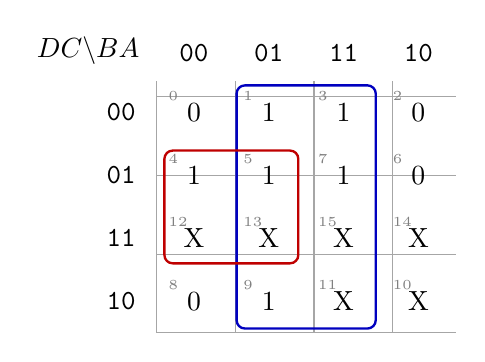
\begin{tikzpicture}[x=0.95cm,y=0.8cm,font=\normalsize]
\draw[gray!70] (0,0) grid (4,4);
\node[anchor=east] at (-0.1,4.48) {$DC\backslash BA$};
\node at (0.5,4.45) {\texttt{00}};
\node[anchor=east] at (-.15,3.5) {\texttt{00}};
\node at (1.5,4.45) {\texttt{01}};
\node[anchor=east] at (-.15,2.5) {\texttt{01}};
\node at (2.5,4.45) {\texttt{11}};
\node[anchor=east] at (-.15,1.5) {\texttt{11}};
\node at (3.5,4.45) {\texttt{10}};
\node[anchor=east] at (-.15,0.5) {\texttt{10}};
\node at (0.5,3.5) {0};
\node[font=\tiny,text=gray,anchor=north west] at (0.03,3.98) {0};
\node at (1.5,3.5) {1};
\node[font=\tiny,text=gray,anchor=north west] at (1.03,3.98) {1};
\node at (2.5,3.5) {1};
\node[font=\tiny,text=gray,anchor=north west] at (2.03,3.98) {3};
\node at (3.5,3.5) {0};
\node[font=\tiny,text=gray,anchor=north west] at (3.03,3.98) {2};
\node at (0.5,2.5) {1};
\node[font=\tiny,text=gray,anchor=north west] at (0.03,2.98) {4};
\node at (1.5,2.5) {1};
\node[font=\tiny,text=gray,anchor=north west] at (1.03,2.98) {5};
\node at (2.5,2.5) {1};
\node[font=\tiny,text=gray,anchor=north west] at (2.03,2.98) {7};
\node at (3.5,2.5) {0};
\node[font=\tiny,text=gray,anchor=north west] at (3.03,2.98) {6};
\node at (0.5,1.5) {X};
\node[font=\tiny,text=gray,anchor=north west] at (0.03,1.98) {12};
\node at (1.5,1.5) {X};
\node[font=\tiny,text=gray,anchor=north west] at (1.03,1.98) {13};
\node at (2.5,1.5) {X};
\node[font=\tiny,text=gray,anchor=north west] at (2.03,1.98) {15};
\node at (3.5,1.5) {X};
\node[font=\tiny,text=gray,anchor=north west] at (3.03,1.98) {14};
\node at (0.5,0.5) {0};
\node[font=\tiny,text=gray,anchor=north west] at (0.03,0.98) {8};
\node at (1.5,0.5) {1};
\node[font=\tiny,text=gray,anchor=north west] at (1.03,0.98) {9};
\node at (2.5,0.5) {X};
\node[font=\tiny,text=gray,anchor=north west] at (2.03,0.98) {11};
\node at (3.5,0.5) {X};
\node[font=\tiny,text=gray,anchor=north west] at (3.03,0.98) {10};
\draw[blue!75!black,line width=.85pt,rounded corners=3pt] (1.07,0.07) rectangle (2.93,3.93);
\draw[red!75!black,line width=.85pt,rounded corners=3pt] (0.10500000000000001,1.105) rectangle (1.895,2.895);
\end{tikzpicture}\end{center}

\begin{center}\small
\begin{tabular}{clll}
\toprule
Group & Cells covered (incl. X) & Fixed variables & Product term\\\midrule
\textcolor{blue!75!black}{$G_{1}$} & $\{1,3,5,7,9,11,13,15\}$ & $A=1$ & $A$\\
\textcolor{red!75!black}{$G_{2}$} & $\{4,5,12,13\}$ & $C=1,B=0$ & $C\overline{B}$\\
\bottomrule\end{tabular}\end{center}


\noindent OR the group terms: $\boxed{e=A + C\overline{B}}$.

\noindent Cost: 2 product term(s), 3 literal(s).

\end{minipage}\par\vspace{0.25cm}

\noindent\begin{minipage}{\textwidth}

\subsection*{BCD: output $f$}

\noindent $f=\sum m\{1,2,3,7\}$; $\mathcal{D}=\{10,11,12,13,14,15\}$.

\begin{center}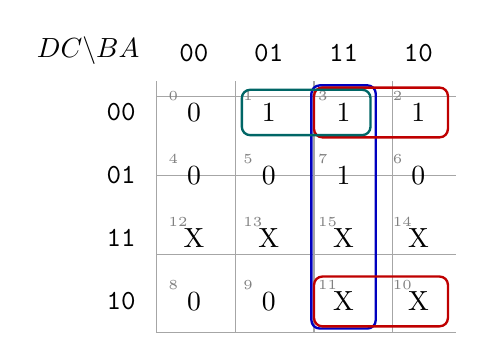
\begin{tikzpicture}[x=0.95cm,y=0.8cm,font=\normalsize]
\draw[gray!70] (0,0) grid (4,4);
\node[anchor=east] at (-0.1,4.48) {$DC\backslash BA$};
\node at (0.5,4.45) {\texttt{00}};
\node[anchor=east] at (-.15,3.5) {\texttt{00}};
\node at (1.5,4.45) {\texttt{01}};
\node[anchor=east] at (-.15,2.5) {\texttt{01}};
\node at (2.5,4.45) {\texttt{11}};
\node[anchor=east] at (-.15,1.5) {\texttt{11}};
\node at (3.5,4.45) {\texttt{10}};
\node[anchor=east] at (-.15,0.5) {\texttt{10}};
\node at (0.5,3.5) {0};
\node[font=\tiny,text=gray,anchor=north west] at (0.03,3.98) {0};
\node at (1.5,3.5) {1};
\node[font=\tiny,text=gray,anchor=north west] at (1.03,3.98) {1};
\node at (2.5,3.5) {1};
\node[font=\tiny,text=gray,anchor=north west] at (2.03,3.98) {3};
\node at (3.5,3.5) {1};
\node[font=\tiny,text=gray,anchor=north west] at (3.03,3.98) {2};
\node at (0.5,2.5) {0};
\node[font=\tiny,text=gray,anchor=north west] at (0.03,2.98) {4};
\node at (1.5,2.5) {0};
\node[font=\tiny,text=gray,anchor=north west] at (1.03,2.98) {5};
\node at (2.5,2.5) {1};
\node[font=\tiny,text=gray,anchor=north west] at (2.03,2.98) {7};
\node at (3.5,2.5) {0};
\node[font=\tiny,text=gray,anchor=north west] at (3.03,2.98) {6};
\node at (0.5,1.5) {X};
\node[font=\tiny,text=gray,anchor=north west] at (0.03,1.98) {12};
\node at (1.5,1.5) {X};
\node[font=\tiny,text=gray,anchor=north west] at (1.03,1.98) {13};
\node at (2.5,1.5) {X};
\node[font=\tiny,text=gray,anchor=north west] at (2.03,1.98) {15};
\node at (3.5,1.5) {X};
\node[font=\tiny,text=gray,anchor=north west] at (3.03,1.98) {14};
\node at (0.5,0.5) {0};
\node[font=\tiny,text=gray,anchor=north west] at (0.03,0.98) {8};
\node at (1.5,0.5) {0};
\node[font=\tiny,text=gray,anchor=north west] at (1.03,0.98) {9};
\node at (2.5,0.5) {X};
\node[font=\tiny,text=gray,anchor=north west] at (2.03,0.98) {11};
\node at (3.5,0.5) {X};
\node[font=\tiny,text=gray,anchor=north west] at (3.03,0.98) {10};
\draw[blue!75!black,line width=.85pt,rounded corners=3pt] (2.07,0.07) rectangle (2.93,3.93);
\draw[red!75!black,line width=.85pt,rounded corners=3pt] (2.105,3.105) rectangle (3.895,3.895);
\draw[red!75!black,line width=.85pt,rounded corners=3pt] (2.105,0.10500000000000001) rectangle (3.895,0.895);
\draw[teal!80!black,line width=.85pt,rounded corners=3pt] (1.1400000000000001,3.14) rectangle (2.86,3.86);
\end{tikzpicture}\end{center}

\begin{center}\small
\begin{tabular}{clll}
\toprule
Group & Cells covered (incl. X) & Fixed variables & Product term\\\midrule
\textcolor{blue!75!black}{$G_{1}$} & $\{3,7,11,15\}$ & $B=1,A=1$ & $BA$\\
\textcolor{red!75!black}{$G_{2}$} & $\{2,3,10,11\}$ & $C=0,B=1$ & $\overline{C}B$\\
\textcolor{teal!80!black}{$G_{3}$} & $\{1,3\}$ & $D=0,C=0,A=1$ & $\overline{D}\overline{C}A$\\
\bottomrule\end{tabular}\end{center}


\noindent OR the group terms: $\boxed{f=BA + \overline{C}B + \overline{D}\overline{C}A}$.

\noindent Cost: 3 product term(s), 7 literal(s).

\end{minipage}\par\vspace{0.25cm}

\clearpage

\noindent\begin{minipage}{\textwidth}

\subsection*{BCD: output $g$}

\noindent $g=\sum m\{0,1,7\}$; $\mathcal{D}=\{10,11,12,13,14,15\}$.

\begin{center}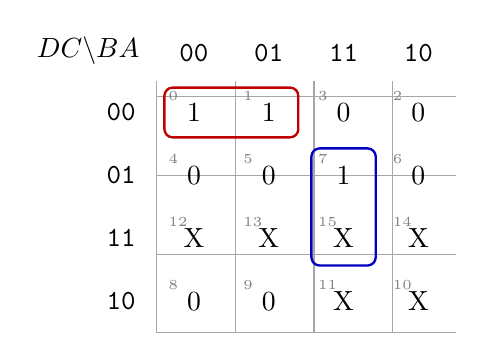
\begin{tikzpicture}[x=0.95cm,y=0.8cm,font=\normalsize]
\draw[gray!70] (0,0) grid (4,4);
\node[anchor=east] at (-0.1,4.48) {$DC\backslash BA$};
\node at (0.5,4.45) {\texttt{00}};
\node[anchor=east] at (-.15,3.5) {\texttt{00}};
\node at (1.5,4.45) {\texttt{01}};
\node[anchor=east] at (-.15,2.5) {\texttt{01}};
\node at (2.5,4.45) {\texttt{11}};
\node[anchor=east] at (-.15,1.5) {\texttt{11}};
\node at (3.5,4.45) {\texttt{10}};
\node[anchor=east] at (-.15,0.5) {\texttt{10}};
\node at (0.5,3.5) {1};
\node[font=\tiny,text=gray,anchor=north west] at (0.03,3.98) {0};
\node at (1.5,3.5) {1};
\node[font=\tiny,text=gray,anchor=north west] at (1.03,3.98) {1};
\node at (2.5,3.5) {0};
\node[font=\tiny,text=gray,anchor=north west] at (2.03,3.98) {3};
\node at (3.5,3.5) {0};
\node[font=\tiny,text=gray,anchor=north west] at (3.03,3.98) {2};
\node at (0.5,2.5) {0};
\node[font=\tiny,text=gray,anchor=north west] at (0.03,2.98) {4};
\node at (1.5,2.5) {0};
\node[font=\tiny,text=gray,anchor=north west] at (1.03,2.98) {5};
\node at (2.5,2.5) {1};
\node[font=\tiny,text=gray,anchor=north west] at (2.03,2.98) {7};
\node at (3.5,2.5) {0};
\node[font=\tiny,text=gray,anchor=north west] at (3.03,2.98) {6};
\node at (0.5,1.5) {X};
\node[font=\tiny,text=gray,anchor=north west] at (0.03,1.98) {12};
\node at (1.5,1.5) {X};
\node[font=\tiny,text=gray,anchor=north west] at (1.03,1.98) {13};
\node at (2.5,1.5) {X};
\node[font=\tiny,text=gray,anchor=north west] at (2.03,1.98) {15};
\node at (3.5,1.5) {X};
\node[font=\tiny,text=gray,anchor=north west] at (3.03,1.98) {14};
\node at (0.5,0.5) {0};
\node[font=\tiny,text=gray,anchor=north west] at (0.03,0.98) {8};
\node at (1.5,0.5) {0};
\node[font=\tiny,text=gray,anchor=north west] at (1.03,0.98) {9};
\node at (2.5,0.5) {X};
\node[font=\tiny,text=gray,anchor=north west] at (2.03,0.98) {11};
\node at (3.5,0.5) {X};
\node[font=\tiny,text=gray,anchor=north west] at (3.03,0.98) {10};
\draw[blue!75!black,line width=.85pt,rounded corners=3pt] (2.07,1.07) rectangle (2.93,2.93);
\draw[red!75!black,line width=.85pt,rounded corners=3pt] (0.10500000000000001,3.105) rectangle (1.895,3.895);
\end{tikzpicture}\end{center}

\begin{center}\small
\begin{tabular}{clll}
\toprule
Group & Cells covered (incl. X) & Fixed variables & Product term\\\midrule
\textcolor{blue!75!black}{$G_{1}$} & $\{7,15\}$ & $C=1,B=1,A=1$ & $CBA$\\
\textcolor{red!75!black}{$G_{2}$} & $\{0,1\}$ & $D=0,C=0,B=0$ & $\overline{D}\overline{C}\overline{B}$\\
\bottomrule\end{tabular}\end{center}


\noindent OR the group terms: $\boxed{g=CBA + \overline{D}\overline{C}\overline{B}}$.

\noindent Cost: 2 product term(s), 6 literal(s).

\end{minipage}\par\vspace{0.25cm}

\clearpage\subsection{BCD decoder: complete gate connections}

Generate $\overline D,\overline C,\overline B,\overline A$ with four shared
inverters, then distribute both polarities of the four inputs. Each row in the left table
defines one product node: use a multi-input AND for a multi-literal term, or a direct wire
for a single literal. The right table gives every output connection. Use an OR gate for
each sum of multiple nodes. These signals are already active-low segment controls;
do not invert all seven outputs again.

\noindent\begin{minipage}[t]{0.47\textwidth}\begin{center}\small
\begin{tabular}{cl}
\toprule
Node & AND inputs / direct wire\\\midrule
$p_{1}$ & $C\overline{B}\overline{A}$\\
$p_{2}$ & $\overline{D}\overline{C}\overline{B}A$\\
$p_{3}$ & $C\overline{B}A$\\
$p_{4}$ & $CB\overline{A}$\\
$p_{5}$ & $\overline{C}B\overline{A}$\\
$p_{6}$ & $CBA$\\
$p_{7}$ & $A$\\
$p_{8}$ & $C\overline{B}$\\
$p_{9}$ & $BA$\\
$p_{10}$ & $\overline{C}B$\\
$p_{11}$ & $\overline{D}\overline{C}A$\\
$p_{12}$ & $\overline{D}\overline{C}\overline{B}$\\
\bottomrule\end{tabular}\end{center}
\end{minipage}\hfill\begin{minipage}[t]{0.49\textwidth}\begin{center}\small
\begin{tabular}{cl}
\toprule
Output & OR inputs / wire\\\midrule
$a$ & $p_{1}+p_{2}$\\
$b$ & $p_{3}+p_{4}$\\
$c$ & $p_{5}$\\
$d$ & $p_{6}+p_{1}+p_{2}$\\
$e$ & $p_{7}+p_{8}$\\
$f$ & $p_{9}+p_{10}+p_{11}$\\
$g$ & $p_{6}+p_{12}$\\
\bottomrule\end{tabular}\end{center}
\end{minipage}

\begin{center}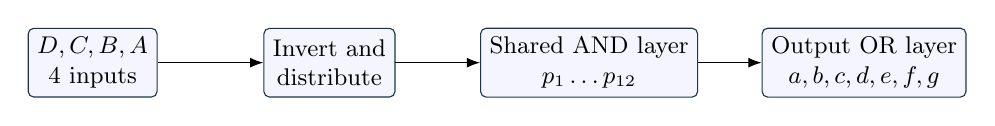
\begin{tikzpicture}[>=Latex,block/.style={draw=ink,rounded corners=2pt,fill=blue!4,minimum height=.9cm,align=center},font=\small,scale=0.97,transform shape]

\node[block] (in) at (0,0) {$D,C,B,A$\\4 inputs};
\node[block] (not) at (3.1,0) {Invert and\\distribute};
\node[block] (and) at (6.5,0) {Shared AND layer\\$p_1\ldots p_{12}$};
\node[block] (or) at (10.1,0) {Output OR layer\\$a,b,c,d,e,f,g$};
\draw[->] (in)--(not);\draw[->] (not)--(and);\draw[->] (and)--(or);

\end{tikzpicture}\end{center}

The block diagram shows the layers; the two tables specify all individual nets. An FPGA maps the logic to LUTs, so discrete gate counts are not Quartus LE counts.

\subsection{Sharing product terms between outputs}
Define
\[
P=C\overline A\overline B,\qquad Q=A\overline B\overline C\overline D,\qquad R=ABC.
\]
Then $a=P+Q$, $d=P+Q+R$, and $g=R+\overline B\overline C\overline D$.
Without sharing, $P$ and $Q$ are each generated separately for a and d; $R$ is generated
separately for d and g. Reusing each of these products saves \textbf{three multi-input
AND gates}, under the convention that one product is implemented by one AND gate.
The input inverters remain shared and the output OR gates are unchanged. For a single
example, sharing $P$ between a and d saves one three-input AND gate.

\clearpage\section{Prelab 2: complete hexadecimal decoder}
Combining digits 0--9 with A, b, C, d, E, and F defines all sixteen rows. There are no
don't-cares. Added rows can require either 0 or 1 for a segment, so a BCD grouping can
become invalid. For example, $C\overline A\overline B$ includes input 12, but glyph C
requires output a to be 0; therefore the corresponding a term needs an additional
$\overline D$ restriction.


\noindent\begin{minipage}{\textwidth}

\subsection*{Hex: output $a$}

\noindent $a=\sum m\{1,4,11,13\}$; no don't-cares.

\begin{center}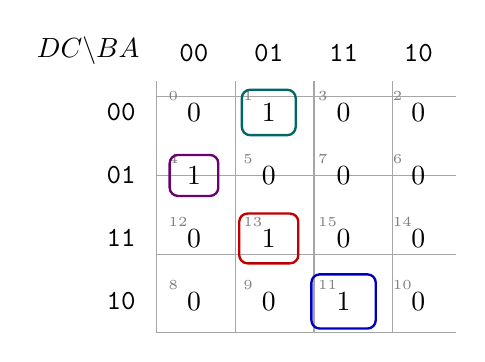
\begin{tikzpicture}[x=0.95cm,y=0.8cm,font=\normalsize]
\draw[gray!70] (0,0) grid (4,4);
\node[anchor=east] at (-0.1,4.48) {$DC\backslash BA$};
\node at (0.5,4.45) {\texttt{00}};
\node[anchor=east] at (-.15,3.5) {\texttt{00}};
\node at (1.5,4.45) {\texttt{01}};
\node[anchor=east] at (-.15,2.5) {\texttt{01}};
\node at (2.5,4.45) {\texttt{11}};
\node[anchor=east] at (-.15,1.5) {\texttt{11}};
\node at (3.5,4.45) {\texttt{10}};
\node[anchor=east] at (-.15,0.5) {\texttt{10}};
\node at (0.5,3.5) {0};
\node[font=\tiny,text=gray,anchor=north west] at (0.03,3.98) {0};
\node at (1.5,3.5) {1};
\node[font=\tiny,text=gray,anchor=north west] at (1.03,3.98) {1};
\node at (2.5,3.5) {0};
\node[font=\tiny,text=gray,anchor=north west] at (2.03,3.98) {3};
\node at (3.5,3.5) {0};
\node[font=\tiny,text=gray,anchor=north west] at (3.03,3.98) {2};
\node at (0.5,2.5) {1};
\node[font=\tiny,text=gray,anchor=north west] at (0.03,2.98) {4};
\node at (1.5,2.5) {0};
\node[font=\tiny,text=gray,anchor=north west] at (1.03,2.98) {5};
\node at (2.5,2.5) {0};
\node[font=\tiny,text=gray,anchor=north west] at (2.03,2.98) {7};
\node at (3.5,2.5) {0};
\node[font=\tiny,text=gray,anchor=north west] at (3.03,2.98) {6};
\node at (0.5,1.5) {0};
\node[font=\tiny,text=gray,anchor=north west] at (0.03,1.98) {12};
\node at (1.5,1.5) {1};
\node[font=\tiny,text=gray,anchor=north west] at (1.03,1.98) {13};
\node at (2.5,1.5) {0};
\node[font=\tiny,text=gray,anchor=north west] at (2.03,1.98) {15};
\node at (3.5,1.5) {0};
\node[font=\tiny,text=gray,anchor=north west] at (3.03,1.98) {14};
\node at (0.5,0.5) {0};
\node[font=\tiny,text=gray,anchor=north west] at (0.03,0.98) {8};
\node at (1.5,0.5) {0};
\node[font=\tiny,text=gray,anchor=north west] at (1.03,0.98) {9};
\node at (2.5,0.5) {1};
\node[font=\tiny,text=gray,anchor=north west] at (2.03,0.98) {11};
\node at (3.5,0.5) {0};
\node[font=\tiny,text=gray,anchor=north west] at (3.03,0.98) {10};
\draw[blue!75!black,line width=.85pt,rounded corners=3pt] (2.07,0.07) rectangle (2.93,0.9299999999999999);
\draw[red!75!black,line width=.85pt,rounded corners=3pt] (1.105,1.105) rectangle (1.895,1.895);
\draw[teal!80!black,line width=.85pt,rounded corners=3pt] (1.1400000000000001,3.14) rectangle (1.8599999999999999,3.86);
\draw[violet!85!black,line width=.85pt,rounded corners=3pt] (0.17500000000000002,2.175) rectangle (0.825,2.825);
\end{tikzpicture}\end{center}

\begin{center}\small
\begin{tabular}{clll}
\toprule
Group & Cells covered (incl. X) & Fixed variables & Product term\\\midrule
\textcolor{blue!75!black}{$G_{1}$} & $\{11\}$ & $D=1,C=0,B=1,A=1$ & $D\overline{C}BA$\\
\textcolor{red!75!black}{$G_{2}$} & $\{13\}$ & $D=1,C=1,B=0,A=1$ & $DC\overline{B}A$\\
\textcolor{teal!80!black}{$G_{3}$} & $\{1\}$ & $D=0,C=0,B=0,A=1$ & $\overline{D}\overline{C}\overline{B}A$\\
\textcolor{violet!85!black}{$G_{4}$} & $\{4\}$ & $D=0,C=1,B=0,A=0$ & $\overline{D}C\overline{B}\overline{A}$\\
\bottomrule\end{tabular}\end{center}


\noindent OR the group terms: $\boxed{a=D\overline{C}BA + DC\overline{B}A + \overline{D}\overline{C}\overline{B}A + \overline{D}C\overline{B}\overline{A}}$.

\noindent Cost: 4 product term(s), 16 literal(s).

\end{minipage}\par\vspace{0.25cm}

\noindent\begin{minipage}{\textwidth}

\subsection*{Hex: output $b$}

\noindent $b=\sum m\{5,6,11,12,14,15\}$; no don't-cares.

\begin{center}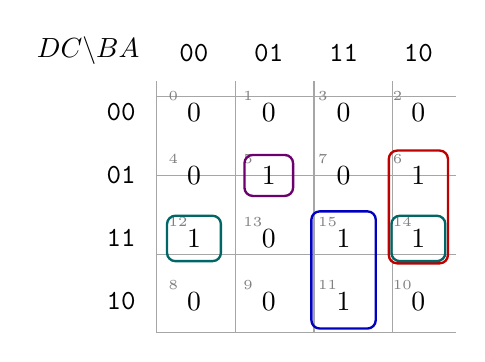
\begin{tikzpicture}[x=0.95cm,y=0.8cm,font=\normalsize]
\draw[gray!70] (0,0) grid (4,4);
\node[anchor=east] at (-0.1,4.48) {$DC\backslash BA$};
\node at (0.5,4.45) {\texttt{00}};
\node[anchor=east] at (-.15,3.5) {\texttt{00}};
\node at (1.5,4.45) {\texttt{01}};
\node[anchor=east] at (-.15,2.5) {\texttt{01}};
\node at (2.5,4.45) {\texttt{11}};
\node[anchor=east] at (-.15,1.5) {\texttt{11}};
\node at (3.5,4.45) {\texttt{10}};
\node[anchor=east] at (-.15,0.5) {\texttt{10}};
\node at (0.5,3.5) {0};
\node[font=\tiny,text=gray,anchor=north west] at (0.03,3.98) {0};
\node at (1.5,3.5) {0};
\node[font=\tiny,text=gray,anchor=north west] at (1.03,3.98) {1};
\node at (2.5,3.5) {0};
\node[font=\tiny,text=gray,anchor=north west] at (2.03,3.98) {3};
\node at (3.5,3.5) {0};
\node[font=\tiny,text=gray,anchor=north west] at (3.03,3.98) {2};
\node at (0.5,2.5) {0};
\node[font=\tiny,text=gray,anchor=north west] at (0.03,2.98) {4};
\node at (1.5,2.5) {1};
\node[font=\tiny,text=gray,anchor=north west] at (1.03,2.98) {5};
\node at (2.5,2.5) {0};
\node[font=\tiny,text=gray,anchor=north west] at (2.03,2.98) {7};
\node at (3.5,2.5) {1};
\node[font=\tiny,text=gray,anchor=north west] at (3.03,2.98) {6};
\node at (0.5,1.5) {1};
\node[font=\tiny,text=gray,anchor=north west] at (0.03,1.98) {12};
\node at (1.5,1.5) {0};
\node[font=\tiny,text=gray,anchor=north west] at (1.03,1.98) {13};
\node at (2.5,1.5) {1};
\node[font=\tiny,text=gray,anchor=north west] at (2.03,1.98) {15};
\node at (3.5,1.5) {1};
\node[font=\tiny,text=gray,anchor=north west] at (3.03,1.98) {14};
\node at (0.5,0.5) {0};
\node[font=\tiny,text=gray,anchor=north west] at (0.03,0.98) {8};
\node at (1.5,0.5) {0};
\node[font=\tiny,text=gray,anchor=north west] at (1.03,0.98) {9};
\node at (2.5,0.5) {1};
\node[font=\tiny,text=gray,anchor=north west] at (2.03,0.98) {11};
\node at (3.5,0.5) {0};
\node[font=\tiny,text=gray,anchor=north west] at (3.03,0.98) {10};
\draw[blue!75!black,line width=.85pt,rounded corners=3pt] (2.07,0.07) rectangle (2.93,1.93);
\draw[red!75!black,line width=.85pt,rounded corners=3pt] (3.105,1.105) rectangle (3.895,2.895);
\draw[teal!80!black,line width=.85pt,rounded corners=3pt] (0.14,1.1400000000000001) rectangle (0.86,1.8599999999999999);
\draw[teal!80!black,line width=.85pt,rounded corners=3pt] (3.14,1.1400000000000001) rectangle (3.86,1.8599999999999999);
\draw[violet!85!black,line width=.85pt,rounded corners=3pt] (1.175,2.175) rectangle (1.825,2.825);
\end{tikzpicture}\end{center}

\begin{center}\small
\begin{tabular}{clll}
\toprule
Group & Cells covered (incl. X) & Fixed variables & Product term\\\midrule
\textcolor{blue!75!black}{$G_{1}$} & $\{11,15\}$ & $D=1,B=1,A=1$ & $DBA$\\
\textcolor{red!75!black}{$G_{2}$} & $\{6,14\}$ & $C=1,B=1,A=0$ & $CB\overline{A}$\\
\textcolor{teal!80!black}{$G_{3}$} & $\{12,14\}$ & $D=1,C=1,A=0$ & $DC\overline{A}$\\
\textcolor{violet!85!black}{$G_{4}$} & $\{5\}$ & $D=0,C=1,B=0,A=1$ & $\overline{D}C\overline{B}A$\\
\bottomrule\end{tabular}\end{center}


\noindent OR the group terms: $\boxed{b=DBA + CB\overline{A} + DC\overline{A} + \overline{D}C\overline{B}A}$.

\noindent Cost: 4 product term(s), 13 literal(s).

\end{minipage}\par\vspace{0.25cm}

\clearpage

\noindent\begin{minipage}{\textwidth}

\subsection*{Hex: output $c$}

\noindent $c=\sum m\{2,12,14,15\}$; no don't-cares.

\begin{center}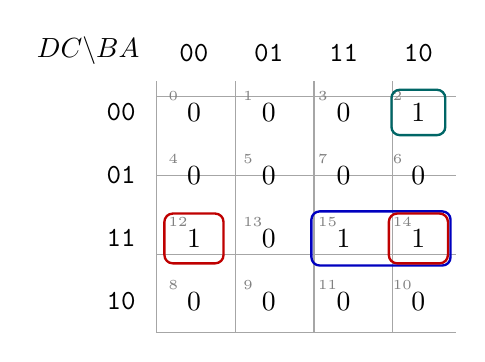
\begin{tikzpicture}[x=0.95cm,y=0.8cm,font=\normalsize]
\draw[gray!70] (0,0) grid (4,4);
\node[anchor=east] at (-0.1,4.48) {$DC\backslash BA$};
\node at (0.5,4.45) {\texttt{00}};
\node[anchor=east] at (-.15,3.5) {\texttt{00}};
\node at (1.5,4.45) {\texttt{01}};
\node[anchor=east] at (-.15,2.5) {\texttt{01}};
\node at (2.5,4.45) {\texttt{11}};
\node[anchor=east] at (-.15,1.5) {\texttt{11}};
\node at (3.5,4.45) {\texttt{10}};
\node[anchor=east] at (-.15,0.5) {\texttt{10}};
\node at (0.5,3.5) {0};
\node[font=\tiny,text=gray,anchor=north west] at (0.03,3.98) {0};
\node at (1.5,3.5) {0};
\node[font=\tiny,text=gray,anchor=north west] at (1.03,3.98) {1};
\node at (2.5,3.5) {0};
\node[font=\tiny,text=gray,anchor=north west] at (2.03,3.98) {3};
\node at (3.5,3.5) {1};
\node[font=\tiny,text=gray,anchor=north west] at (3.03,3.98) {2};
\node at (0.5,2.5) {0};
\node[font=\tiny,text=gray,anchor=north west] at (0.03,2.98) {4};
\node at (1.5,2.5) {0};
\node[font=\tiny,text=gray,anchor=north west] at (1.03,2.98) {5};
\node at (2.5,2.5) {0};
\node[font=\tiny,text=gray,anchor=north west] at (2.03,2.98) {7};
\node at (3.5,2.5) {0};
\node[font=\tiny,text=gray,anchor=north west] at (3.03,2.98) {6};
\node at (0.5,1.5) {1};
\node[font=\tiny,text=gray,anchor=north west] at (0.03,1.98) {12};
\node at (1.5,1.5) {0};
\node[font=\tiny,text=gray,anchor=north west] at (1.03,1.98) {13};
\node at (2.5,1.5) {1};
\node[font=\tiny,text=gray,anchor=north west] at (2.03,1.98) {15};
\node at (3.5,1.5) {1};
\node[font=\tiny,text=gray,anchor=north west] at (3.03,1.98) {14};
\node at (0.5,0.5) {0};
\node[font=\tiny,text=gray,anchor=north west] at (0.03,0.98) {8};
\node at (1.5,0.5) {0};
\node[font=\tiny,text=gray,anchor=north west] at (1.03,0.98) {9};
\node at (2.5,0.5) {0};
\node[font=\tiny,text=gray,anchor=north west] at (2.03,0.98) {11};
\node at (3.5,0.5) {0};
\node[font=\tiny,text=gray,anchor=north west] at (3.03,0.98) {10};
\draw[blue!75!black,line width=.85pt,rounded corners=3pt] (2.07,1.07) rectangle (3.93,1.93);
\draw[red!75!black,line width=.85pt,rounded corners=3pt] (0.10500000000000001,1.105) rectangle (0.895,1.895);
\draw[red!75!black,line width=.85pt,rounded corners=3pt] (3.105,1.105) rectangle (3.895,1.895);
\draw[teal!80!black,line width=.85pt,rounded corners=3pt] (3.14,3.14) rectangle (3.86,3.86);
\end{tikzpicture}\end{center}

\begin{center}\small
\begin{tabular}{clll}
\toprule
Group & Cells covered (incl. X) & Fixed variables & Product term\\\midrule
\textcolor{blue!75!black}{$G_{1}$} & $\{14,15\}$ & $D=1,C=1,B=1$ & $DCB$\\
\textcolor{red!75!black}{$G_{2}$} & $\{12,14\}$ & $D=1,C=1,A=0$ & $DC\overline{A}$\\
\textcolor{teal!80!black}{$G_{3}$} & $\{2\}$ & $D=0,C=0,B=1,A=0$ & $\overline{D}\overline{C}B\overline{A}$\\
\bottomrule\end{tabular}\end{center}


\noindent OR the group terms: $\boxed{c=DCB + DC\overline{A} + \overline{D}\overline{C}B\overline{A}}$.

\noindent Cost: 3 product term(s), 10 literal(s).

\end{minipage}\par\vspace{0.25cm}

\noindent\begin{minipage}{\textwidth}

\subsection*{Hex: output $d$}

\noindent $d=\sum m\{1,4,7,10,15\}$; no don't-cares.

\begin{center}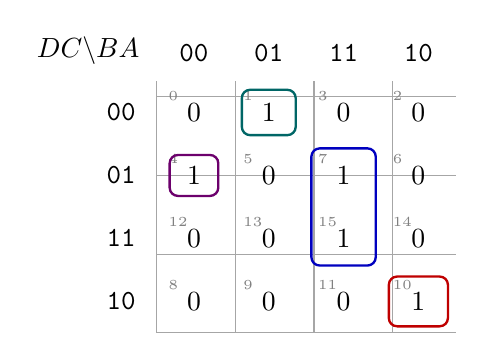
\begin{tikzpicture}[x=0.95cm,y=0.8cm,font=\normalsize]
\draw[gray!70] (0,0) grid (4,4);
\node[anchor=east] at (-0.1,4.48) {$DC\backslash BA$};
\node at (0.5,4.45) {\texttt{00}};
\node[anchor=east] at (-.15,3.5) {\texttt{00}};
\node at (1.5,4.45) {\texttt{01}};
\node[anchor=east] at (-.15,2.5) {\texttt{01}};
\node at (2.5,4.45) {\texttt{11}};
\node[anchor=east] at (-.15,1.5) {\texttt{11}};
\node at (3.5,4.45) {\texttt{10}};
\node[anchor=east] at (-.15,0.5) {\texttt{10}};
\node at (0.5,3.5) {0};
\node[font=\tiny,text=gray,anchor=north west] at (0.03,3.98) {0};
\node at (1.5,3.5) {1};
\node[font=\tiny,text=gray,anchor=north west] at (1.03,3.98) {1};
\node at (2.5,3.5) {0};
\node[font=\tiny,text=gray,anchor=north west] at (2.03,3.98) {3};
\node at (3.5,3.5) {0};
\node[font=\tiny,text=gray,anchor=north west] at (3.03,3.98) {2};
\node at (0.5,2.5) {1};
\node[font=\tiny,text=gray,anchor=north west] at (0.03,2.98) {4};
\node at (1.5,2.5) {0};
\node[font=\tiny,text=gray,anchor=north west] at (1.03,2.98) {5};
\node at (2.5,2.5) {1};
\node[font=\tiny,text=gray,anchor=north west] at (2.03,2.98) {7};
\node at (3.5,2.5) {0};
\node[font=\tiny,text=gray,anchor=north west] at (3.03,2.98) {6};
\node at (0.5,1.5) {0};
\node[font=\tiny,text=gray,anchor=north west] at (0.03,1.98) {12};
\node at (1.5,1.5) {0};
\node[font=\tiny,text=gray,anchor=north west] at (1.03,1.98) {13};
\node at (2.5,1.5) {1};
\node[font=\tiny,text=gray,anchor=north west] at (2.03,1.98) {15};
\node at (3.5,1.5) {0};
\node[font=\tiny,text=gray,anchor=north west] at (3.03,1.98) {14};
\node at (0.5,0.5) {0};
\node[font=\tiny,text=gray,anchor=north west] at (0.03,0.98) {8};
\node at (1.5,0.5) {0};
\node[font=\tiny,text=gray,anchor=north west] at (1.03,0.98) {9};
\node at (2.5,0.5) {0};
\node[font=\tiny,text=gray,anchor=north west] at (2.03,0.98) {11};
\node at (3.5,0.5) {1};
\node[font=\tiny,text=gray,anchor=north west] at (3.03,0.98) {10};
\draw[blue!75!black,line width=.85pt,rounded corners=3pt] (2.07,1.07) rectangle (2.93,2.93);
\draw[red!75!black,line width=.85pt,rounded corners=3pt] (3.105,0.10500000000000001) rectangle (3.895,0.895);
\draw[teal!80!black,line width=.85pt,rounded corners=3pt] (1.1400000000000001,3.14) rectangle (1.8599999999999999,3.86);
\draw[violet!85!black,line width=.85pt,rounded corners=3pt] (0.17500000000000002,2.175) rectangle (0.825,2.825);
\end{tikzpicture}\end{center}

\begin{center}\small
\begin{tabular}{clll}
\toprule
Group & Cells covered (incl. X) & Fixed variables & Product term\\\midrule
\textcolor{blue!75!black}{$G_{1}$} & $\{7,15\}$ & $C=1,B=1,A=1$ & $CBA$\\
\textcolor{red!75!black}{$G_{2}$} & $\{10\}$ & $D=1,C=0,B=1,A=0$ & $D\overline{C}B\overline{A}$\\
\textcolor{teal!80!black}{$G_{3}$} & $\{1\}$ & $D=0,C=0,B=0,A=1$ & $\overline{D}\overline{C}\overline{B}A$\\
\textcolor{violet!85!black}{$G_{4}$} & $\{4\}$ & $D=0,C=1,B=0,A=0$ & $\overline{D}C\overline{B}\overline{A}$\\
\bottomrule\end{tabular}\end{center}


\noindent OR the group terms: $\boxed{d=CBA + D\overline{C}B\overline{A} + \overline{D}\overline{C}\overline{B}A + \overline{D}C\overline{B}\overline{A}}$.

\noindent Cost: 4 product term(s), 15 literal(s).

\end{minipage}\par\vspace{0.25cm}

\clearpage

\noindent\begin{minipage}{\textwidth}

\subsection*{Hex: output $e$}

\noindent $e=\sum m\{1,3,4,5,7,9\}$; no don't-cares.

\begin{center}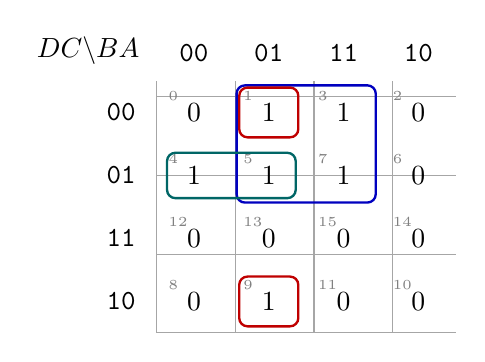
\begin{tikzpicture}[x=0.95cm,y=0.8cm,font=\normalsize]
\draw[gray!70] (0,0) grid (4,4);
\node[anchor=east] at (-0.1,4.48) {$DC\backslash BA$};
\node at (0.5,4.45) {\texttt{00}};
\node[anchor=east] at (-.15,3.5) {\texttt{00}};
\node at (1.5,4.45) {\texttt{01}};
\node[anchor=east] at (-.15,2.5) {\texttt{01}};
\node at (2.5,4.45) {\texttt{11}};
\node[anchor=east] at (-.15,1.5) {\texttt{11}};
\node at (3.5,4.45) {\texttt{10}};
\node[anchor=east] at (-.15,0.5) {\texttt{10}};
\node at (0.5,3.5) {0};
\node[font=\tiny,text=gray,anchor=north west] at (0.03,3.98) {0};
\node at (1.5,3.5) {1};
\node[font=\tiny,text=gray,anchor=north west] at (1.03,3.98) {1};
\node at (2.5,3.5) {1};
\node[font=\tiny,text=gray,anchor=north west] at (2.03,3.98) {3};
\node at (3.5,3.5) {0};
\node[font=\tiny,text=gray,anchor=north west] at (3.03,3.98) {2};
\node at (0.5,2.5) {1};
\node[font=\tiny,text=gray,anchor=north west] at (0.03,2.98) {4};
\node at (1.5,2.5) {1};
\node[font=\tiny,text=gray,anchor=north west] at (1.03,2.98) {5};
\node at (2.5,2.5) {1};
\node[font=\tiny,text=gray,anchor=north west] at (2.03,2.98) {7};
\node at (3.5,2.5) {0};
\node[font=\tiny,text=gray,anchor=north west] at (3.03,2.98) {6};
\node at (0.5,1.5) {0};
\node[font=\tiny,text=gray,anchor=north west] at (0.03,1.98) {12};
\node at (1.5,1.5) {0};
\node[font=\tiny,text=gray,anchor=north west] at (1.03,1.98) {13};
\node at (2.5,1.5) {0};
\node[font=\tiny,text=gray,anchor=north west] at (2.03,1.98) {15};
\node at (3.5,1.5) {0};
\node[font=\tiny,text=gray,anchor=north west] at (3.03,1.98) {14};
\node at (0.5,0.5) {0};
\node[font=\tiny,text=gray,anchor=north west] at (0.03,0.98) {8};
\node at (1.5,0.5) {1};
\node[font=\tiny,text=gray,anchor=north west] at (1.03,0.98) {9};
\node at (2.5,0.5) {0};
\node[font=\tiny,text=gray,anchor=north west] at (2.03,0.98) {11};
\node at (3.5,0.5) {0};
\node[font=\tiny,text=gray,anchor=north west] at (3.03,0.98) {10};
\draw[blue!75!black,line width=.85pt,rounded corners=3pt] (1.07,2.07) rectangle (2.93,3.93);
\draw[red!75!black,line width=.85pt,rounded corners=3pt] (1.105,3.105) rectangle (1.895,3.895);
\draw[red!75!black,line width=.85pt,rounded corners=3pt] (1.105,0.10500000000000001) rectangle (1.895,0.895);
\draw[teal!80!black,line width=.85pt,rounded corners=3pt] (0.14,2.14) rectangle (1.8599999999999999,2.86);
\end{tikzpicture}\end{center}

\begin{center}\small
\begin{tabular}{clll}
\toprule
Group & Cells covered (incl. X) & Fixed variables & Product term\\\midrule
\textcolor{blue!75!black}{$G_{1}$} & $\{1,3,5,7\}$ & $D=0,A=1$ & $\overline{D}A$\\
\textcolor{red!75!black}{$G_{2}$} & $\{1,9\}$ & $C=0,B=0,A=1$ & $\overline{C}\overline{B}A$\\
\textcolor{teal!80!black}{$G_{3}$} & $\{4,5\}$ & $D=0,C=1,B=0$ & $\overline{D}C\overline{B}$\\
\bottomrule\end{tabular}\end{center}


\noindent OR the group terms: $\boxed{e=\overline{D}A + \overline{C}\overline{B}A + \overline{D}C\overline{B}}$.

\noindent Cost: 3 product term(s), 8 literal(s).

\end{minipage}\par\vspace{0.25cm}

\noindent\begin{minipage}{\textwidth}

\subsection*{Hex: output $f$}

\noindent $f=\sum m\{1,2,3,7,13\}$; no don't-cares.

\begin{center}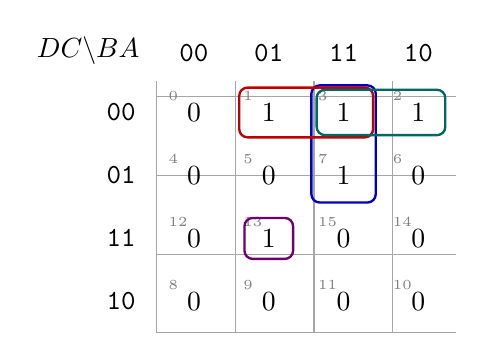
\begin{tikzpicture}[x=0.95cm,y=0.8cm,font=\normalsize]
\draw[gray!70] (0,0) grid (4,4);
\node[anchor=east] at (-0.1,4.48) {$DC\backslash BA$};
\node at (0.5,4.45) {\texttt{00}};
\node[anchor=east] at (-.15,3.5) {\texttt{00}};
\node at (1.5,4.45) {\texttt{01}};
\node[anchor=east] at (-.15,2.5) {\texttt{01}};
\node at (2.5,4.45) {\texttt{11}};
\node[anchor=east] at (-.15,1.5) {\texttt{11}};
\node at (3.5,4.45) {\texttt{10}};
\node[anchor=east] at (-.15,0.5) {\texttt{10}};
\node at (0.5,3.5) {0};
\node[font=\tiny,text=gray,anchor=north west] at (0.03,3.98) {0};
\node at (1.5,3.5) {1};
\node[font=\tiny,text=gray,anchor=north west] at (1.03,3.98) {1};
\node at (2.5,3.5) {1};
\node[font=\tiny,text=gray,anchor=north west] at (2.03,3.98) {3};
\node at (3.5,3.5) {1};
\node[font=\tiny,text=gray,anchor=north west] at (3.03,3.98) {2};
\node at (0.5,2.5) {0};
\node[font=\tiny,text=gray,anchor=north west] at (0.03,2.98) {4};
\node at (1.5,2.5) {0};
\node[font=\tiny,text=gray,anchor=north west] at (1.03,2.98) {5};
\node at (2.5,2.5) {1};
\node[font=\tiny,text=gray,anchor=north west] at (2.03,2.98) {7};
\node at (3.5,2.5) {0};
\node[font=\tiny,text=gray,anchor=north west] at (3.03,2.98) {6};
\node at (0.5,1.5) {0};
\node[font=\tiny,text=gray,anchor=north west] at (0.03,1.98) {12};
\node at (1.5,1.5) {1};
\node[font=\tiny,text=gray,anchor=north west] at (1.03,1.98) {13};
\node at (2.5,1.5) {0};
\node[font=\tiny,text=gray,anchor=north west] at (2.03,1.98) {15};
\node at (3.5,1.5) {0};
\node[font=\tiny,text=gray,anchor=north west] at (3.03,1.98) {14};
\node at (0.5,0.5) {0};
\node[font=\tiny,text=gray,anchor=north west] at (0.03,0.98) {8};
\node at (1.5,0.5) {0};
\node[font=\tiny,text=gray,anchor=north west] at (1.03,0.98) {9};
\node at (2.5,0.5) {0};
\node[font=\tiny,text=gray,anchor=north west] at (2.03,0.98) {11};
\node at (3.5,0.5) {0};
\node[font=\tiny,text=gray,anchor=north west] at (3.03,0.98) {10};
\draw[blue!75!black,line width=.85pt,rounded corners=3pt] (2.07,2.07) rectangle (2.93,3.93);
\draw[red!75!black,line width=.85pt,rounded corners=3pt] (1.105,3.105) rectangle (2.895,3.895);
\draw[teal!80!black,line width=.85pt,rounded corners=3pt] (2.14,3.14) rectangle (3.86,3.86);
\draw[violet!85!black,line width=.85pt,rounded corners=3pt] (1.175,1.175) rectangle (1.825,1.825);
\end{tikzpicture}\end{center}

\begin{center}\small
\begin{tabular}{clll}
\toprule
Group & Cells covered (incl. X) & Fixed variables & Product term\\\midrule
\textcolor{blue!75!black}{$G_{1}$} & $\{3,7\}$ & $D=0,B=1,A=1$ & $\overline{D}BA$\\
\textcolor{red!75!black}{$G_{2}$} & $\{1,3\}$ & $D=0,C=0,A=1$ & $\overline{D}\overline{C}A$\\
\textcolor{teal!80!black}{$G_{3}$} & $\{2,3\}$ & $D=0,C=0,B=1$ & $\overline{D}\overline{C}B$\\
\textcolor{violet!85!black}{$G_{4}$} & $\{13\}$ & $D=1,C=1,B=0,A=1$ & $DC\overline{B}A$\\
\bottomrule\end{tabular}\end{center}


\noindent OR the group terms: $\boxed{f=\overline{D}BA + \overline{D}\overline{C}A + \overline{D}\overline{C}B + DC\overline{B}A}$.

\noindent Cost: 4 product term(s), 13 literal(s).

\end{minipage}\par\vspace{0.25cm}

\clearpage

\noindent\begin{minipage}{\textwidth}

\subsection*{Hex: output $g$}

\noindent $g=\sum m\{0,1,7,12\}$; no don't-cares.

\begin{center}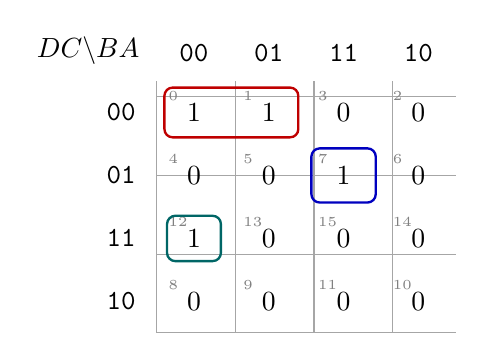
\begin{tikzpicture}[x=0.95cm,y=0.8cm,font=\normalsize]
\draw[gray!70] (0,0) grid (4,4);
\node[anchor=east] at (-0.1,4.48) {$DC\backslash BA$};
\node at (0.5,4.45) {\texttt{00}};
\node[anchor=east] at (-.15,3.5) {\texttt{00}};
\node at (1.5,4.45) {\texttt{01}};
\node[anchor=east] at (-.15,2.5) {\texttt{01}};
\node at (2.5,4.45) {\texttt{11}};
\node[anchor=east] at (-.15,1.5) {\texttt{11}};
\node at (3.5,4.45) {\texttt{10}};
\node[anchor=east] at (-.15,0.5) {\texttt{10}};
\node at (0.5,3.5) {1};
\node[font=\tiny,text=gray,anchor=north west] at (0.03,3.98) {0};
\node at (1.5,3.5) {1};
\node[font=\tiny,text=gray,anchor=north west] at (1.03,3.98) {1};
\node at (2.5,3.5) {0};
\node[font=\tiny,text=gray,anchor=north west] at (2.03,3.98) {3};
\node at (3.5,3.5) {0};
\node[font=\tiny,text=gray,anchor=north west] at (3.03,3.98) {2};
\node at (0.5,2.5) {0};
\node[font=\tiny,text=gray,anchor=north west] at (0.03,2.98) {4};
\node at (1.5,2.5) {0};
\node[font=\tiny,text=gray,anchor=north west] at (1.03,2.98) {5};
\node at (2.5,2.5) {1};
\node[font=\tiny,text=gray,anchor=north west] at (2.03,2.98) {7};
\node at (3.5,2.5) {0};
\node[font=\tiny,text=gray,anchor=north west] at (3.03,2.98) {6};
\node at (0.5,1.5) {1};
\node[font=\tiny,text=gray,anchor=north west] at (0.03,1.98) {12};
\node at (1.5,1.5) {0};
\node[font=\tiny,text=gray,anchor=north west] at (1.03,1.98) {13};
\node at (2.5,1.5) {0};
\node[font=\tiny,text=gray,anchor=north west] at (2.03,1.98) {15};
\node at (3.5,1.5) {0};
\node[font=\tiny,text=gray,anchor=north west] at (3.03,1.98) {14};
\node at (0.5,0.5) {0};
\node[font=\tiny,text=gray,anchor=north west] at (0.03,0.98) {8};
\node at (1.5,0.5) {0};
\node[font=\tiny,text=gray,anchor=north west] at (1.03,0.98) {9};
\node at (2.5,0.5) {0};
\node[font=\tiny,text=gray,anchor=north west] at (2.03,0.98) {11};
\node at (3.5,0.5) {0};
\node[font=\tiny,text=gray,anchor=north west] at (3.03,0.98) {10};
\draw[blue!75!black,line width=.85pt,rounded corners=3pt] (2.07,2.07) rectangle (2.93,2.93);
\draw[red!75!black,line width=.85pt,rounded corners=3pt] (0.10500000000000001,3.105) rectangle (1.895,3.895);
\draw[teal!80!black,line width=.85pt,rounded corners=3pt] (0.14,1.1400000000000001) rectangle (0.86,1.8599999999999999);
\end{tikzpicture}\end{center}

\begin{center}\small
\begin{tabular}{clll}
\toprule
Group & Cells covered (incl. X) & Fixed variables & Product term\\\midrule
\textcolor{blue!75!black}{$G_{1}$} & $\{7\}$ & $D=0,C=1,B=1,A=1$ & $\overline{D}CBA$\\
\textcolor{red!75!black}{$G_{2}$} & $\{0,1\}$ & $D=0,C=0,B=0$ & $\overline{D}\overline{C}\overline{B}$\\
\textcolor{teal!80!black}{$G_{3}$} & $\{12\}$ & $D=1,C=1,B=0,A=0$ & $DC\overline{B}\overline{A}$\\
\bottomrule\end{tabular}\end{center}


\noindent OR the group terms: $\boxed{g=\overline{D}CBA + \overline{D}\overline{C}\overline{B} + DC\overline{B}\overline{A}}$.

\noindent Cost: 3 product term(s), 11 literal(s).

\end{minipage}\par\vspace{0.25cm}

\clearpage\subsection{hex7seg: complete gate connections}

Generate $\overline D,\overline C,\overline B,\overline A$ with four shared
inverters, then distribute both polarities of the four inputs. Each row in the left table
defines one product node: use a multi-input AND for a multi-literal term, or a direct wire
for a single literal. The right table gives every output connection. Use an OR gate for
each sum of multiple nodes. These signals are already active-low segment controls;
do not invert all seven outputs again.

\noindent\begin{minipage}[t]{0.47\textwidth}\begin{center}\small
\begin{tabular}{cl}
\toprule
Node & AND inputs / direct wire\\\midrule
$q_{1}$ & $D\overline{C}BA$\\
$q_{2}$ & $DC\overline{B}A$\\
$q_{3}$ & $\overline{D}\overline{C}\overline{B}A$\\
$q_{4}$ & $\overline{D}C\overline{B}\overline{A}$\\
$q_{5}$ & $DBA$\\
$q_{6}$ & $CB\overline{A}$\\
$q_{7}$ & $DC\overline{A}$\\
$q_{8}$ & $\overline{D}C\overline{B}A$\\
$q_{9}$ & $DCB$\\
$q_{10}$ & $\overline{D}\overline{C}B\overline{A}$\\
$q_{11}$ & $CBA$\\
$q_{12}$ & $D\overline{C}B\overline{A}$\\
$q_{13}$ & $\overline{D}A$\\
$q_{14}$ & $\overline{C}\overline{B}A$\\
$q_{15}$ & $\overline{D}C\overline{B}$\\
$q_{16}$ & $\overline{D}BA$\\
$q_{17}$ & $\overline{D}\overline{C}A$\\
$q_{18}$ & $\overline{D}\overline{C}B$\\
$q_{19}$ & $\overline{D}CBA$\\
$q_{20}$ & $\overline{D}\overline{C}\overline{B}$\\
$q_{21}$ & $DC\overline{B}\overline{A}$\\
\bottomrule\end{tabular}\end{center}
\end{minipage}\hfill\begin{minipage}[t]{0.49\textwidth}\begin{center}\small
\begin{tabular}{cl}
\toprule
Output & OR inputs / wire\\\midrule
$a$ & $q_{1}+q_{2}+q_{3}+q_{4}$\\
$b$ & $q_{5}+q_{6}+q_{7}+q_{8}$\\
$c$ & $q_{9}+q_{7}+q_{10}$\\
$d$ & $q_{11}+q_{12}+q_{3}+q_{4}$\\
$e$ & $q_{13}+q_{14}+q_{15}$\\
$f$ & $q_{16}+q_{17}+q_{18}+q_{2}$\\
$g$ & $q_{19}+q_{20}+q_{21}$\\
\bottomrule\end{tabular}\end{center}
\end{minipage}

\begin{center}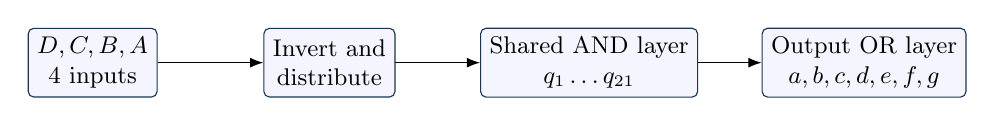
\begin{tikzpicture}[>=Latex,block/.style={draw=ink,rounded corners=2pt,fill=blue!4,minimum height=.9cm,align=center},font=\small,scale=0.97,transform shape]

\node[block] (in) at (0,0) {$D,C,B,A$\\4 inputs};
\node[block] (not) at (3.1,0) {Invert and\\distribute};
\node[block] (and) at (6.5,0) {Shared AND layer\\$q_1\ldots q_{21}$};
\node[block] (or) at (10.1,0) {Output OR layer\\$a,b,c,d,e,f,g$};
\draw[->] (in)--(not);\draw[->] (not)--(and);\draw[->] (and)--(or);

\end{tikzpicture}\end{center}

The block diagram shows the layers; the two tables specify all individual nets. An FPGA maps the logic to LUTs, so discrete gate counts are not Quartus LE counts.

\clearpage\subsection{Cost comparison}

\begin{center}\small
\begin{tabular}{ccccc}
\toprule
Output & BCD terms & Hex terms & BCD literals & Hex literals\\\midrule
$a$ & 2 & 4 & 7 & 16\\
$b$ & 2 & 4 & 6 & 13\\
$c$ & 1 & 3 & 3 & 10\\
$d$ & 3 & 4 & 10 & 15\\
$e$ & 2 & 3 & 3 & 8\\
$f$ & 3 & 4 & 7 & 13\\
$g$ & 2 & 3 & 6 & 11\\
Total & 15 & 25 & 42 & 86\\
\bottomrule\end{tabular}\end{center}


\begin{center}\small
\begin{tabular}{lcc}
\toprule
After identical-term sharing & BCD & Hex\\\midrule
Distinct product nodes (including direct wires) & 12 & 21\\
Multi-input AND gates & 11 & 21\\
Multi-input OR gates & 6 & 7\\
Input inverters & 4 & 4\\
Product-layer literals after sharing & 32 & 71\\
Quartus Total logic elements & \pending & \pending\\
\bottomrule\end{tabular}\end{center}


A literal is one occurrence of an input variable or its complement in a product;
OR connections are not counted as literals. Gate counts assume arbitrary fan-in.
The BCD term $A$ is a direct wire, not an AND gate. Exact FPGA LE counts cannot be
inferred from these abstract counts.

Experiment 1 also fixes $D=0$, enabling further synthesis simplification. Consequently,
its LE difference from Experiment 2 reflects both the input restriction and the
decoder change. A controlled BCD-versus-Hex comparison would retain four input ports,
the same FPGA target, and the same synthesis settings.
\subsection{Concrete gate circuit for hexadecimal segment a}


\begin{center}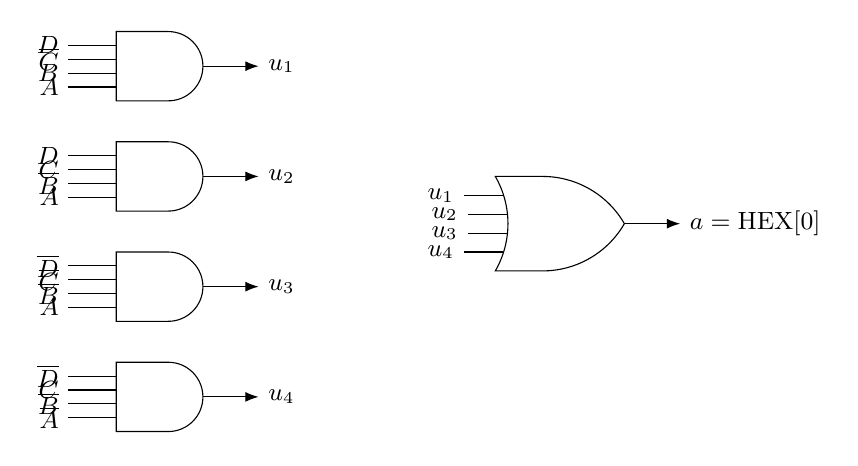
\begin{tikzpicture}[>=Latex,block/.style={draw=ink,rounded corners=2pt,fill=blue!4,minimum height=.9cm,align=center},font=\small,scale=1,transform shape]
\node[and gate US,draw,logic gate inputs=nnnn,minimum width=1.1cm,minimum height=.75cm] (g0) at (4,3.0) {};
\draw (g0.input 1) -- ++(-.6,0) node[left] {$D$};
\draw (g0.input 2) -- ++(-.6,0) node[left] {$\overline{C}$};
\draw (g0.input 3) -- ++(-.6,0) node[left] {$B$};
\draw (g0.input 4) -- ++(-.6,0) node[left] {$A$};
\draw[->] (g0.output) -- ++(.7,0) node[right] {$u_{1}$};
\node[and gate US,draw,logic gate inputs=nnnn,minimum width=1.1cm,minimum height=.75cm] (g1) at (4,1.6) {};
\draw (g1.input 1) -- ++(-.6,0) node[left] {$D$};
\draw (g1.input 2) -- ++(-.6,0) node[left] {$C$};
\draw (g1.input 3) -- ++(-.6,0) node[left] {$\overline{B}$};
\draw (g1.input 4) -- ++(-.6,0) node[left] {$A$};
\draw[->] (g1.output) -- ++(.7,0) node[right] {$u_{2}$};
\node[and gate US,draw,logic gate inputs=nnnn,minimum width=1.1cm,minimum height=.75cm] (g2) at (4,0.20000000000000018) {};
\draw (g2.input 1) -- ++(-.6,0) node[left] {$\overline{D}$};
\draw (g2.input 2) -- ++(-.6,0) node[left] {$\overline{C}$};
\draw (g2.input 3) -- ++(-.6,0) node[left] {$\overline{B}$};
\draw (g2.input 4) -- ++(-.6,0) node[left] {$A$};
\draw[->] (g2.output) -- ++(.7,0) node[right] {$u_{3}$};
\node[and gate US,draw,logic gate inputs=nnnn,minimum width=1.1cm,minimum height=.75cm] (g3) at (4,-1.1999999999999993) {};
\draw (g3.input 1) -- ++(-.6,0) node[left] {$\overline{D}$};
\draw (g3.input 2) -- ++(-.6,0) node[left] {$C$};
\draw (g3.input 3) -- ++(-.6,0) node[left] {$\overline{B}$};
\draw (g3.input 4) -- ++(-.6,0) node[left] {$\overline{A}$};
\draw[->] (g3.output) -- ++(.7,0) node[right] {$u_{4}$};
\node[or gate US,draw,logic gate inputs=nnnn,minimum width=1.1cm,minimum height=1.2cm] (og) at (9,1) {};
\draw (og.input 1) -- ++(-.5,0) node[left] {$u_{1}$};
\draw (og.input 2) -- ++(-.5,0) node[left] {$u_{2}$};
\draw (og.input 3) -- ++(-.5,0) node[left] {$u_{3}$};
\draw (og.input 4) -- ++(-.5,0) node[left] {$u_{4}$};
\draw[->] (og.output) -- ++(.7,0) node[right] {$a=\mathrm{HEX}[0]$};
\end{tikzpicture}\end{center}

The four $u_i$ nets correspond, in order, to the four terms in the a expression.
Matching labels denote the same net. Construct the other six outputs using the full
connection tables; shared product nodes feed multiple output gates.

\clearpage\subsection{Theoretical timing for all sixteen codes}
The diagram below is a \textbf{zero-delay theoretical waveform}, not a ModelSim
screenshot. Start every input at 0 at $t=0$. Use periods of 20, 40, 80, and 160 ns for
$d_0,d_1,d_2,d_3$, each with a 50\% duty cycle. A new input code appears every 10 ns,
covering all sixteen codes during $[0,160)$ ns.


\begin{center}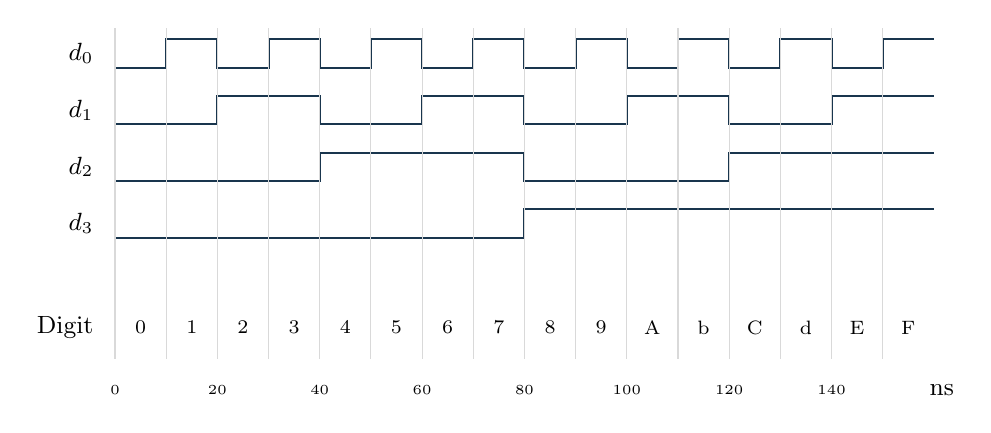
\begin{tikzpicture}[>=Latex,block/.style={draw=ink,rounded corners=2pt,fill=blue!4,minimum height=.9cm,align=center},font=\small,scale=1,transform shape]
\node[anchor=east] at (-.15,4.18) {$d_0$};
\draw[ink,line width=.7pt] (0,4.0) -- (0.65,4.0) -- (0.65,4.36) -- (1.3,4.36) -- (1.3,4.0) -- (1.9500000000000002,4.0) -- (1.9500000000000002,4.36) -- (2.6,4.36) -- (2.6,4.0) -- (3.25,4.0) -- (3.25,4.36) -- (3.9000000000000004,4.36) -- (3.9000000000000004,4.0) -- (4.55,4.0) -- (4.55,4.36) -- (5.2,4.36) -- (5.2,4.0) -- (5.8500000000000005,4.0) -- (5.8500000000000005,4.36) -- (6.5,4.36) -- (6.5,4.0) -- (7.15,4.0) -- (7.15,4.36) -- (7.800000000000001,4.36) -- (7.800000000000001,4.0) -- (8.450000000000001,4.0) -- (8.450000000000001,4.36) -- (9.1,4.36) -- (9.1,4.0) -- (9.75,4.0) -- (9.75,4.36) -- (10.4,4.36);
\node[anchor=east] at (-.15,3.4600000000000004) {$d_1$};
\draw[ink,line width=.7pt] (0,3.2800000000000002) -- (0.65,3.2800000000000002) -- (1.3,3.2800000000000002) -- (1.3,3.64) -- (1.9500000000000002,3.64) -- (2.6,3.64) -- (2.6,3.2800000000000002) -- (3.25,3.2800000000000002) -- (3.9000000000000004,3.2800000000000002) -- (3.9000000000000004,3.64) -- (4.55,3.64) -- (5.2,3.64) -- (5.2,3.2800000000000002) -- (5.8500000000000005,3.2800000000000002) -- (6.5,3.2800000000000002) -- (6.5,3.64) -- (7.15,3.64) -- (7.800000000000001,3.64) -- (7.800000000000001,3.2800000000000002) -- (8.450000000000001,3.2800000000000002) -- (9.1,3.2800000000000002) -- (9.1,3.64) -- (9.75,3.64) -- (10.4,3.64);
\node[anchor=east] at (-.15,2.74) {$d_2$};
\draw[ink,line width=.7pt] (0,2.56) -- (0.65,2.56) -- (1.3,2.56) -- (1.9500000000000002,2.56) -- (2.6,2.56) -- (2.6,2.92) -- (3.25,2.92) -- (3.9000000000000004,2.92) -- (4.55,2.92) -- (5.2,2.92) -- (5.2,2.56) -- (5.8500000000000005,2.56) -- (6.5,2.56) -- (7.15,2.56) -- (7.800000000000001,2.56) -- (7.800000000000001,2.92) -- (8.450000000000001,2.92) -- (9.1,2.92) -- (9.75,2.92) -- (10.4,2.92);
\node[anchor=east] at (-.15,2.02) {$d_3$};
\draw[ink,line width=.7pt] (0,1.8399999999999999) -- (0.65,1.8399999999999999) -- (1.3,1.8399999999999999) -- (1.9500000000000002,1.8399999999999999) -- (2.6,1.8399999999999999) -- (3.25,1.8399999999999999) -- (3.9000000000000004,1.8399999999999999) -- (4.55,1.8399999999999999) -- (5.2,1.8399999999999999) -- (5.2,2.1999999999999997) -- (5.8500000000000005,2.1999999999999997) -- (6.5,2.1999999999999997) -- (7.15,2.1999999999999997) -- (7.800000000000001,2.1999999999999997) -- (8.450000000000001,2.1999999999999997) -- (9.1,2.1999999999999997) -- (9.75,2.1999999999999997) -- (10.4,2.1999999999999997);
\draw[gray!30] (0.0,0.3)--(0.0,4.5);
\node[font=\scriptsize] at (0.325,.7) {0};
\node[font=\tiny] at (0.0,-.1) {0};
\draw[gray!30] (0.65,0.3)--(0.65,4.5);
\node[font=\scriptsize] at (0.9750000000000001,.7) {1};
\draw[gray!30] (1.3,0.3)--(1.3,4.5);
\node[font=\scriptsize] at (1.625,.7) {2};
\node[font=\tiny] at (1.3,-.1) {20};
\draw[gray!30] (1.9500000000000002,0.3)--(1.9500000000000002,4.5);
\node[font=\scriptsize] at (2.2750000000000004,.7) {3};
\draw[gray!30] (2.6,0.3)--(2.6,4.5);
\node[font=\scriptsize] at (2.9250000000000003,.7) {4};
\node[font=\tiny] at (2.6,-.1) {40};
\draw[gray!30] (3.25,0.3)--(3.25,4.5);
\node[font=\scriptsize] at (3.575,.7) {5};
\draw[gray!30] (3.9000000000000004,0.3)--(3.9000000000000004,4.5);
\node[font=\scriptsize] at (4.2250000000000005,.7) {6};
\node[font=\tiny] at (3.9000000000000004,-.1) {60};
\draw[gray!30] (4.55,0.3)--(4.55,4.5);
\node[font=\scriptsize] at (4.875,.7) {7};
\draw[gray!30] (5.2,0.3)--(5.2,4.5);
\node[font=\scriptsize] at (5.525,.7) {8};
\node[font=\tiny] at (5.2,-.1) {80};
\draw[gray!30] (5.8500000000000005,0.3)--(5.8500000000000005,4.5);
\node[font=\scriptsize] at (6.175000000000001,.7) {9};
\draw[gray!30] (6.5,0.3)--(6.5,4.5);
\node[font=\scriptsize] at (6.825,.7) {A};
\node[font=\tiny] at (6.5,-.1) {100};
\draw[gray!30] (7.15,0.3)--(7.15,4.5);
\node[font=\scriptsize] at (7.4750000000000005,.7) {b};
\draw[gray!30] (7.800000000000001,0.3)--(7.800000000000001,4.5);
\node[font=\scriptsize] at (8.125,.7) {C};
\node[font=\tiny] at (7.800000000000001,-.1) {120};
\draw[gray!30] (8.450000000000001,0.3)--(8.450000000000001,4.5);
\node[font=\scriptsize] at (8.775,.7) {d};
\draw[gray!30] (9.1,0.3)--(9.1,4.5);
\node[font=\scriptsize] at (9.424999999999999,.7) {E};
\node[font=\tiny] at (9.1,-.1) {140};
\draw[gray!30] (9.75,0.3)--(9.75,4.5);
\node[font=\scriptsize] at (10.075,.7) {F};
\node[anchor=east] at (-.15,.7) {Digit};\node at (10.5,-.1) {ns};
\end{tikzpicture}\end{center}

\begin{center}\small
\begin{tabular}{cccc}
\toprule
Interval / ns & $DCBA$ & Expected glyph & Expected $abcdefg$\\\midrule
$[0,10)$ & \texttt{0000} & 0 & \texttt{0000001}\\
$[10,20)$ & \texttt{0001} & 1 & \texttt{1001111}\\
$[20,30)$ & \texttt{0010} & 2 & \texttt{0010010}\\
$[30,40)$ & \texttt{0011} & 3 & \texttt{0000110}\\
$[40,50)$ & \texttt{0100} & 4 & \texttt{1001100}\\
$[50,60)$ & \texttt{0101} & 5 & \texttt{0100100}\\
$[60,70)$ & \texttt{0110} & 6 & \texttt{0100000}\\
$[70,80)$ & \texttt{0111} & 7 & \texttt{0001111}\\
$[80,90)$ & \texttt{1000} & 8 & \texttt{0000000}\\
$[90,100)$ & \texttt{1001} & 9 & \texttt{0000100}\\
$[100,110)$ & \texttt{1010} & A & \texttt{0001000}\\
$[110,120)$ & \texttt{1011} & b & \texttt{1100000}\\
$[120,130)$ & \texttt{1100} & C & \texttt{0110001}\\
$[130,140)$ & \texttt{1101} & d & \texttt{1000010}\\
$[140,150)$ & \texttt{1110} & E & \texttt{0110000}\\
$[150,160)$ & \texttt{1111} & F & \texttt{0111000}\\
\bottomrule\end{tabular}\end{center}


In a real simulation, sample after the combinational circuit settles, for
example at $5,15,\ldots,155$ ns. Different initial clock levels or phases change the
order of the codes; always interpret the input bus rather than assuming an order.

\clearpage\section{Prelab 3: result and operation-letter displays}
\subsection{Letter patterns and select logic}
Use the operation codes from Lab 8. Lowercase o uses segments c, d, e, and g, distinguishing
it from digit 0.


\begin{center}\small
\begin{tabular}{ccccc}
\toprule
$S_1S_0$ & Operation & Letter & Lit segments & $abcdefg$\\\midrule
00 & AND & A & a,b,c,e,f,g & \texttt{0001000}\\
01 & OR & o & c,d,e,g & \texttt{1100010}\\
10 & XOR & E & a,d,e,f,g & \texttt{0110000}\\
11 & ADD & d & b,c,d,e,g & \texttt{1000010}\\
\bottomrule\end{tabular}\end{center}


Let the HEX1 segment outputs be $\ell_a,\ldots,\ell_g$. Reading each column
of the four-row truth table gives
\begin{align*}
\ell_a&=S_0,&\ell_b&=S_1\oplus S_0,&\ell_c&=S_1\overline{S_0},\\
\ell_d&=\overline{S_1}\,\overline{S_0},&\ell_e&=0,&\ell_f&=S_0,&\ell_g&=0.
\end{align*}
For example, $\ell_c=1$ only for $S_1S_0=10$ (E); c is lit for the other letters.
Thus $\ell_c=S_1\overline{S_0}$. Outputs $\ell_a$ and $\ell_f$ share the $S_0$ wire.


\begin{center}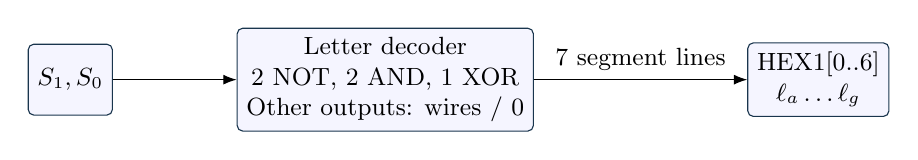
\begin{tikzpicture}[>=Latex,block/.style={draw=ink,rounded corners=2pt,fill=blue!4,minimum height=.9cm,align=center},font=\small,scale=1,transform shape]

\node[block] (s) at (0,0) {$S_1,S_0$};
\node[block] (l) at (4,0) {Letter decoder\\2 NOT, 2 AND, 1 XOR\\Other outputs: wires / 0};
\node[block] (h) at (9.5,0) {HEX1[0..6]\\$\ell_a\ldots\ell_g$};
\draw[->] (s)--(l);\draw[->] (l)-- node[above] {7 segment lines} (h);

\end{tikzpicture}\end{center}

Alternatively, use seven 4:1 multiplexers, one per segment. All share
$S_1,S_0$. Connect each column's four constants to $I_0,I_1,I_2,I_3$ in that order.
For a, the constants are $(0,1,0,1)$; for b, $(0,1,1,0)$; e and g are always 0.
\subsection{Alternative retaining a second hex7seg}\label{sec:lettervariant}
If two \texttt{hex7seg} instances are required at the top level, let the second initially
decode A, 0, E, and d. For $S_1S_0=00,01,10,11$, supply $1010,0000,1110,1101$,
respectively. The encoding logic is
\[
D_L=S_1+\overline{S_0},\quad C_L=S_1,\quad B_L=\overline{S_0},\quad A_L=S_1S_0.
\]
Let $q=\overline{S_1}S_0$, which is 1 only for OR, and let the second decoder outputs
be $h_a,\ldots,h_g$. Override the outputs as follows:
\[
\ell_a=h_a+q,\quad\ell_b=h_b+q,\quad\ell_f=h_f+q,\quad\ell_g=h_g\overline q,
\qquad\ell_c=h_c,\ \ell_d=h_d,\ \ell_e=h_e.
\]
For OR, this turns a, b, and f off and g on, changing 0 to o. The other three glyphs pass
unchanged. \textbf{Only the final override outputs drive HEX1; never connect two output
drivers together.} This alternative costs extra logic; the primary design uses the
direct letter decoder.

\clearpage\section{Prelab 4: binary-to-Gray and BCD-to-excess-3}
\subsection{Deriving the four Gray-code equations}
Let the binary input be $b_3b_2b_1b_0$. The most significant Gray bit equals the binary
MSB. Each remaining Gray bit indicates whether two neighboring binary bits differ:
\[
\boxed{g_3=b_3,\quad g_2=b_3\oplus b_2,\quad g_1=b_2\oplus b_1,\quad g_0=b_1\oplus b_0.}
\]
The XOR truth table is $00\mapsto0$, $01\mapsto1$, $10\mapsto1$, $11\mapsto0$.
Equal neighboring bits give 0; unequal bits give 1. In vector form,
$G=B\oplus(B\!\gg\!1)$. The circuit needs \textbf{three XOR gates and one direct wire};
no K-map is needed.


\begin{center}\begin{tikzpicture}[>=Latex,block/.style={draw=ink,rounded corners=2pt,fill=blue!4,minimum height=.9cm,align=center},font=\small,scale=1,transform shape]

\draw[->] (0,3)--(7,3) node[right] {$g_3$};\node[left] at (0,3) {$b_3$};
\node[xor gate US,draw,logic gate inputs=nn,minimum width=1.2cm] (x2) at (5,1.7) {};
\node[xor gate US,draw,logic gate inputs=nn,minimum width=1.2cm] (x1) at (5,.2) {};
\node[xor gate US,draw,logic gate inputs=nn,minimum width=1.2cm] (x0) at (5,-1.3) {};
\draw (x2.input 1)--++(-1.2,0) node[left] {$b_3$};\draw (x2.input 2)--++(-1.2,0) node[left] {$b_2$};
\draw (x1.input 1)--++(-1.2,0) node[left] {$b_2$};\draw (x1.input 2)--++(-1.2,0) node[left] {$b_1$};
\draw (x0.input 1)--++(-1.2,0) node[left] {$b_1$};\draw (x0.input 2)--++(-1.2,0) node[left] {$b_0$};
\draw[->] (x2.output)--++(1.2,0) node[right] {$g_2$};
\draw[->] (x1.output)--++(1.2,0) node[right] {$g_1$};
\draw[->] (x0.output)--++(1.2,0) node[right] {$g_0$};

\end{tikzpicture}\end{center}

\subsection{Excess-3 truth table and bit-by-bit minimization}
Valid inputs are BCD digits 0--9. The target is $Z=\operatorname{value}(DCBA)+3$;
inputs 10--15 are don't-cares. Write the output as $z_3z_2z_1z_0$.


\begin{center}\small
\begin{tabular}{ccccc}
\toprule
Decimal & $DCBA$ & $z_3z_2z_1z_0$ & Hex glyph & Arithmetic\\\midrule
0 & \texttt{0000} & \texttt{0011} & 3 & $0+3=3$\\
1 & \texttt{0001} & \texttt{0100} & 4 & $1+3=4$\\
2 & \texttt{0010} & \texttt{0101} & 5 & $2+3=5$\\
3 & \texttt{0011} & \texttt{0110} & 6 & $3+3=6$\\
4 & \texttt{0100} & \texttt{0111} & 7 & $4+3=7$\\
5 & \texttt{0101} & \texttt{1000} & 8 & $5+3=8$\\
6 & \texttt{0110} & \texttt{1001} & 9 & $6+3=9$\\
7 & \texttt{0111} & \texttt{1010} & A & $7+3=10$\\
8 & \texttt{1000} & \texttt{1011} & b & $8+3=11$\\
9 & \texttt{1001} & \texttt{1100} & C & $9+3=12$\\
\bottomrule\end{tabular}\end{center}


\clearpage

\noindent\begin{minipage}{\textwidth}

\subsection*{Excess-3: output $z_3$}

\noindent $z_3=\sum m\{5,6,7,8,9\}$; $\mathcal{D}=\{10,11,12,13,14,15\}$.

\begin{center}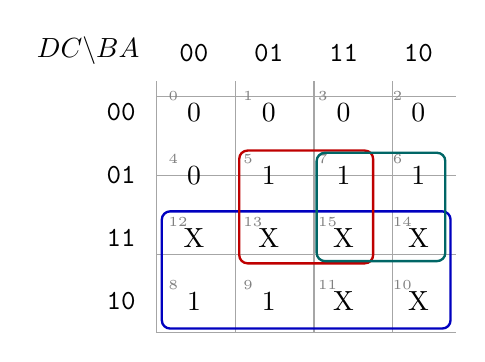
\begin{tikzpicture}[x=0.95cm,y=0.8cm,font=\normalsize]
\draw[gray!70] (0,0) grid (4,4);
\node[anchor=east] at (-0.1,4.48) {$DC\backslash BA$};
\node at (0.5,4.45) {\texttt{00}};
\node[anchor=east] at (-.15,3.5) {\texttt{00}};
\node at (1.5,4.45) {\texttt{01}};
\node[anchor=east] at (-.15,2.5) {\texttt{01}};
\node at (2.5,4.45) {\texttt{11}};
\node[anchor=east] at (-.15,1.5) {\texttt{11}};
\node at (3.5,4.45) {\texttt{10}};
\node[anchor=east] at (-.15,0.5) {\texttt{10}};
\node at (0.5,3.5) {0};
\node[font=\tiny,text=gray,anchor=north west] at (0.03,3.98) {0};
\node at (1.5,3.5) {0};
\node[font=\tiny,text=gray,anchor=north west] at (1.03,3.98) {1};
\node at (2.5,3.5) {0};
\node[font=\tiny,text=gray,anchor=north west] at (2.03,3.98) {3};
\node at (3.5,3.5) {0};
\node[font=\tiny,text=gray,anchor=north west] at (3.03,3.98) {2};
\node at (0.5,2.5) {0};
\node[font=\tiny,text=gray,anchor=north west] at (0.03,2.98) {4};
\node at (1.5,2.5) {1};
\node[font=\tiny,text=gray,anchor=north west] at (1.03,2.98) {5};
\node at (2.5,2.5) {1};
\node[font=\tiny,text=gray,anchor=north west] at (2.03,2.98) {7};
\node at (3.5,2.5) {1};
\node[font=\tiny,text=gray,anchor=north west] at (3.03,2.98) {6};
\node at (0.5,1.5) {X};
\node[font=\tiny,text=gray,anchor=north west] at (0.03,1.98) {12};
\node at (1.5,1.5) {X};
\node[font=\tiny,text=gray,anchor=north west] at (1.03,1.98) {13};
\node at (2.5,1.5) {X};
\node[font=\tiny,text=gray,anchor=north west] at (2.03,1.98) {15};
\node at (3.5,1.5) {X};
\node[font=\tiny,text=gray,anchor=north west] at (3.03,1.98) {14};
\node at (0.5,0.5) {1};
\node[font=\tiny,text=gray,anchor=north west] at (0.03,0.98) {8};
\node at (1.5,0.5) {1};
\node[font=\tiny,text=gray,anchor=north west] at (1.03,0.98) {9};
\node at (2.5,0.5) {X};
\node[font=\tiny,text=gray,anchor=north west] at (2.03,0.98) {11};
\node at (3.5,0.5) {X};
\node[font=\tiny,text=gray,anchor=north west] at (3.03,0.98) {10};
\draw[blue!75!black,line width=.85pt,rounded corners=3pt] (0.07,0.07) rectangle (3.93,1.93);
\draw[red!75!black,line width=.85pt,rounded corners=3pt] (1.105,1.105) rectangle (2.895,2.895);
\draw[teal!80!black,line width=.85pt,rounded corners=3pt] (2.14,1.1400000000000001) rectangle (3.86,2.86);
\end{tikzpicture}\end{center}

\begin{center}\small
\begin{tabular}{clll}
\toprule
Group & Cells covered (incl. X) & Fixed variables & Product term\\\midrule
\textcolor{blue!75!black}{$G_{1}$} & $\{8,9,10,11,12,13,14,15\}$ & $D=1$ & $D$\\
\textcolor{red!75!black}{$G_{2}$} & $\{5,7,13,15\}$ & $C=1,A=1$ & $CA$\\
\textcolor{teal!80!black}{$G_{3}$} & $\{6,7,14,15\}$ & $C=1,B=1$ & $CB$\\
\bottomrule\end{tabular}\end{center}


\noindent OR the group terms: $\boxed{z_3=D + CA + CB}$.

\noindent Cost: 3 product term(s), 5 literal(s).

\end{minipage}\par\vspace{0.25cm}

\noindent\begin{minipage}{\textwidth}

\subsection*{Excess-3: output $z_2$}

\noindent $z_2=\sum m\{1,2,3,4,9\}$; $\mathcal{D}=\{10,11,12,13,14,15\}$.

\begin{center}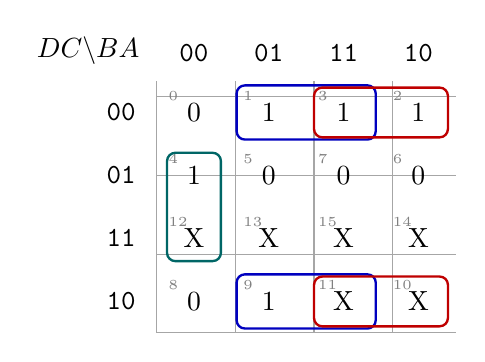
\begin{tikzpicture}[x=0.95cm,y=0.8cm,font=\normalsize]
\draw[gray!70] (0,0) grid (4,4);
\node[anchor=east] at (-0.1,4.48) {$DC\backslash BA$};
\node at (0.5,4.45) {\texttt{00}};
\node[anchor=east] at (-.15,3.5) {\texttt{00}};
\node at (1.5,4.45) {\texttt{01}};
\node[anchor=east] at (-.15,2.5) {\texttt{01}};
\node at (2.5,4.45) {\texttt{11}};
\node[anchor=east] at (-.15,1.5) {\texttt{11}};
\node at (3.5,4.45) {\texttt{10}};
\node[anchor=east] at (-.15,0.5) {\texttt{10}};
\node at (0.5,3.5) {0};
\node[font=\tiny,text=gray,anchor=north west] at (0.03,3.98) {0};
\node at (1.5,3.5) {1};
\node[font=\tiny,text=gray,anchor=north west] at (1.03,3.98) {1};
\node at (2.5,3.5) {1};
\node[font=\tiny,text=gray,anchor=north west] at (2.03,3.98) {3};
\node at (3.5,3.5) {1};
\node[font=\tiny,text=gray,anchor=north west] at (3.03,3.98) {2};
\node at (0.5,2.5) {1};
\node[font=\tiny,text=gray,anchor=north west] at (0.03,2.98) {4};
\node at (1.5,2.5) {0};
\node[font=\tiny,text=gray,anchor=north west] at (1.03,2.98) {5};
\node at (2.5,2.5) {0};
\node[font=\tiny,text=gray,anchor=north west] at (2.03,2.98) {7};
\node at (3.5,2.5) {0};
\node[font=\tiny,text=gray,anchor=north west] at (3.03,2.98) {6};
\node at (0.5,1.5) {X};
\node[font=\tiny,text=gray,anchor=north west] at (0.03,1.98) {12};
\node at (1.5,1.5) {X};
\node[font=\tiny,text=gray,anchor=north west] at (1.03,1.98) {13};
\node at (2.5,1.5) {X};
\node[font=\tiny,text=gray,anchor=north west] at (2.03,1.98) {15};
\node at (3.5,1.5) {X};
\node[font=\tiny,text=gray,anchor=north west] at (3.03,1.98) {14};
\node at (0.5,0.5) {0};
\node[font=\tiny,text=gray,anchor=north west] at (0.03,0.98) {8};
\node at (1.5,0.5) {1};
\node[font=\tiny,text=gray,anchor=north west] at (1.03,0.98) {9};
\node at (2.5,0.5) {X};
\node[font=\tiny,text=gray,anchor=north west] at (2.03,0.98) {11};
\node at (3.5,0.5) {X};
\node[font=\tiny,text=gray,anchor=north west] at (3.03,0.98) {10};
\draw[blue!75!black,line width=.85pt,rounded corners=3pt] (1.07,3.07) rectangle (2.93,3.93);
\draw[blue!75!black,line width=.85pt,rounded corners=3pt] (1.07,0.07) rectangle (2.93,0.9299999999999999);
\draw[red!75!black,line width=.85pt,rounded corners=3pt] (2.105,3.105) rectangle (3.895,3.895);
\draw[red!75!black,line width=.85pt,rounded corners=3pt] (2.105,0.10500000000000001) rectangle (3.895,0.895);
\draw[teal!80!black,line width=.85pt,rounded corners=3pt] (0.14,1.1400000000000001) rectangle (0.86,2.86);
\end{tikzpicture}\end{center}

\begin{center}\small
\begin{tabular}{clll}
\toprule
Group & Cells covered (incl. X) & Fixed variables & Product term\\\midrule
\textcolor{blue!75!black}{$G_{1}$} & $\{1,3,9,11\}$ & $C=0,A=1$ & $\overline{C}A$\\
\textcolor{red!75!black}{$G_{2}$} & $\{2,3,10,11\}$ & $C=0,B=1$ & $\overline{C}B$\\
\textcolor{teal!80!black}{$G_{3}$} & $\{4,12\}$ & $C=1,B=0,A=0$ & $C\overline{B}\overline{A}$\\
\bottomrule\end{tabular}\end{center}


\noindent OR the group terms: $\boxed{z_2=\overline{C}A + \overline{C}B + C\overline{B}\overline{A}}$.

\noindent Cost: 3 product term(s), 7 literal(s).

\end{minipage}\par\vspace{0.25cm}

\clearpage

\noindent\begin{minipage}{\textwidth}

\subsection*{Excess-3: output $z_1$}

\noindent $z_1=\sum m\{0,3,4,7,8\}$; $\mathcal{D}=\{10,11,12,13,14,15\}$.

\begin{center}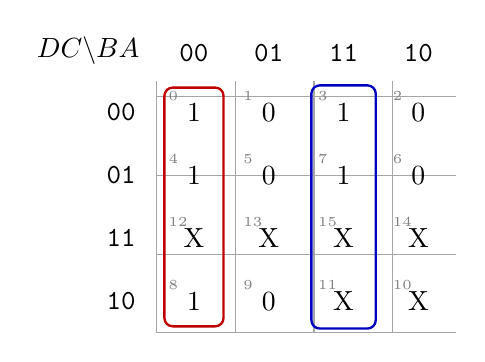
\begin{tikzpicture}[x=0.95cm,y=0.8cm,font=\normalsize]
\draw[gray!70] (0,0) grid (4,4);
\node[anchor=east] at (-0.1,4.48) {$DC\backslash BA$};
\node at (0.5,4.45) {\texttt{00}};
\node[anchor=east] at (-.15,3.5) {\texttt{00}};
\node at (1.5,4.45) {\texttt{01}};
\node[anchor=east] at (-.15,2.5) {\texttt{01}};
\node at (2.5,4.45) {\texttt{11}};
\node[anchor=east] at (-.15,1.5) {\texttt{11}};
\node at (3.5,4.45) {\texttt{10}};
\node[anchor=east] at (-.15,0.5) {\texttt{10}};
\node at (0.5,3.5) {1};
\node[font=\tiny,text=gray,anchor=north west] at (0.03,3.98) {0};
\node at (1.5,3.5) {0};
\node[font=\tiny,text=gray,anchor=north west] at (1.03,3.98) {1};
\node at (2.5,3.5) {1};
\node[font=\tiny,text=gray,anchor=north west] at (2.03,3.98) {3};
\node at (3.5,3.5) {0};
\node[font=\tiny,text=gray,anchor=north west] at (3.03,3.98) {2};
\node at (0.5,2.5) {1};
\node[font=\tiny,text=gray,anchor=north west] at (0.03,2.98) {4};
\node at (1.5,2.5) {0};
\node[font=\tiny,text=gray,anchor=north west] at (1.03,2.98) {5};
\node at (2.5,2.5) {1};
\node[font=\tiny,text=gray,anchor=north west] at (2.03,2.98) {7};
\node at (3.5,2.5) {0};
\node[font=\tiny,text=gray,anchor=north west] at (3.03,2.98) {6};
\node at (0.5,1.5) {X};
\node[font=\tiny,text=gray,anchor=north west] at (0.03,1.98) {12};
\node at (1.5,1.5) {X};
\node[font=\tiny,text=gray,anchor=north west] at (1.03,1.98) {13};
\node at (2.5,1.5) {X};
\node[font=\tiny,text=gray,anchor=north west] at (2.03,1.98) {15};
\node at (3.5,1.5) {X};
\node[font=\tiny,text=gray,anchor=north west] at (3.03,1.98) {14};
\node at (0.5,0.5) {1};
\node[font=\tiny,text=gray,anchor=north west] at (0.03,0.98) {8};
\node at (1.5,0.5) {0};
\node[font=\tiny,text=gray,anchor=north west] at (1.03,0.98) {9};
\node at (2.5,0.5) {X};
\node[font=\tiny,text=gray,anchor=north west] at (2.03,0.98) {11};
\node at (3.5,0.5) {X};
\node[font=\tiny,text=gray,anchor=north west] at (3.03,0.98) {10};
\draw[blue!75!black,line width=.85pt,rounded corners=3pt] (2.07,0.07) rectangle (2.93,3.93);
\draw[red!75!black,line width=.85pt,rounded corners=3pt] (0.10500000000000001,0.10500000000000001) rectangle (0.895,3.895);
\end{tikzpicture}\end{center}

\begin{center}\small
\begin{tabular}{clll}
\toprule
Group & Cells covered (incl. X) & Fixed variables & Product term\\\midrule
\textcolor{blue!75!black}{$G_{1}$} & $\{3,7,11,15\}$ & $B=1,A=1$ & $BA$\\
\textcolor{red!75!black}{$G_{2}$} & $\{0,4,8,12\}$ & $B=0,A=0$ & $\overline{B}\overline{A}$\\
\bottomrule\end{tabular}\end{center}


\noindent OR the group terms: $\boxed{z_1=BA + \overline{B}\overline{A}}$.

\noindent Cost: 2 product term(s), 4 literal(s).

\end{minipage}\par\vspace{0.25cm}

\noindent\begin{minipage}{\textwidth}

\subsection*{Excess-3: output $z_0$}

\noindent $z_0=\sum m\{0,2,4,6,8\}$; $\mathcal{D}=\{10,11,12,13,14,15\}$.

\begin{center}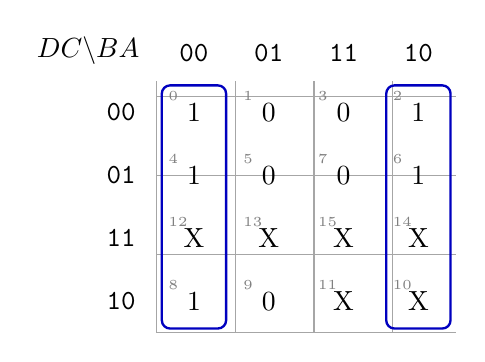
\begin{tikzpicture}[x=0.95cm,y=0.8cm,font=\normalsize]
\draw[gray!70] (0,0) grid (4,4);
\node[anchor=east] at (-0.1,4.48) {$DC\backslash BA$};
\node at (0.5,4.45) {\texttt{00}};
\node[anchor=east] at (-.15,3.5) {\texttt{00}};
\node at (1.5,4.45) {\texttt{01}};
\node[anchor=east] at (-.15,2.5) {\texttt{01}};
\node at (2.5,4.45) {\texttt{11}};
\node[anchor=east] at (-.15,1.5) {\texttt{11}};
\node at (3.5,4.45) {\texttt{10}};
\node[anchor=east] at (-.15,0.5) {\texttt{10}};
\node at (0.5,3.5) {1};
\node[font=\tiny,text=gray,anchor=north west] at (0.03,3.98) {0};
\node at (1.5,3.5) {0};
\node[font=\tiny,text=gray,anchor=north west] at (1.03,3.98) {1};
\node at (2.5,3.5) {0};
\node[font=\tiny,text=gray,anchor=north west] at (2.03,3.98) {3};
\node at (3.5,3.5) {1};
\node[font=\tiny,text=gray,anchor=north west] at (3.03,3.98) {2};
\node at (0.5,2.5) {1};
\node[font=\tiny,text=gray,anchor=north west] at (0.03,2.98) {4};
\node at (1.5,2.5) {0};
\node[font=\tiny,text=gray,anchor=north west] at (1.03,2.98) {5};
\node at (2.5,2.5) {0};
\node[font=\tiny,text=gray,anchor=north west] at (2.03,2.98) {7};
\node at (3.5,2.5) {1};
\node[font=\tiny,text=gray,anchor=north west] at (3.03,2.98) {6};
\node at (0.5,1.5) {X};
\node[font=\tiny,text=gray,anchor=north west] at (0.03,1.98) {12};
\node at (1.5,1.5) {X};
\node[font=\tiny,text=gray,anchor=north west] at (1.03,1.98) {13};
\node at (2.5,1.5) {X};
\node[font=\tiny,text=gray,anchor=north west] at (2.03,1.98) {15};
\node at (3.5,1.5) {X};
\node[font=\tiny,text=gray,anchor=north west] at (3.03,1.98) {14};
\node at (0.5,0.5) {1};
\node[font=\tiny,text=gray,anchor=north west] at (0.03,0.98) {8};
\node at (1.5,0.5) {0};
\node[font=\tiny,text=gray,anchor=north west] at (1.03,0.98) {9};
\node at (2.5,0.5) {X};
\node[font=\tiny,text=gray,anchor=north west] at (2.03,0.98) {11};
\node at (3.5,0.5) {X};
\node[font=\tiny,text=gray,anchor=north west] at (3.03,0.98) {10};
\draw[blue!75!black,line width=.85pt,rounded corners=3pt] (0.07,0.07) rectangle (0.9299999999999999,3.93);
\draw[blue!75!black,line width=.85pt,rounded corners=3pt] (3.07,0.07) rectangle (3.93,3.93);
\end{tikzpicture}\end{center}

\begin{center}\small
\begin{tabular}{clll}
\toprule
Group & Cells covered (incl. X) & Fixed variables & Product term\\\midrule
\textcolor{blue!75!black}{$G_{1}$} & $\{0,2,4,6,8,10,12,14\}$ & $A=0$ & $\overline{A}$\\
\bottomrule\end{tabular}\end{center}


\noindent OR the group terms: $\boxed{z_0=\overline{A}}$.

\noindent Cost: 1 product term(s), 1 literal(s).

\end{minipage}\par\vspace{0.25cm}

\clearpage\subsection{Complete excess-3 connections}
Combining the four maps gives
\begin{align*}
z_3&=D+AC+BC=D+C(A+B),\\
z_2&=A\overline C+B\overline C+C\overline A\overline B
      =\overline C(A+B)+C\overline{(A+B)}=C\oplus(A+B),\\
z_1&=AB+\overline A\overline B=\overline{A\oplus B},\\
z_0&=\overline A.
\end{align*}
Introduce $T=A+B$ and $U=CT$ to reuse intermediate logic. These equations are specified
for valid BCD inputs only: \textbf{inputs 10--15 are not required to produce input plus 3}.


\begin{center}\small
\begin{tabular}{cll}
\toprule
Node & Gate / connection & Destination\\\midrule
$T$ & $\operatorname{OR}(A,B)$ & AND input for $U$; XOR input for $z_2$\\
$U$ & $\operatorname{AND}(C,T)$ & OR input for $z_3$\\
$z_3$ & $\operatorname{OR}(D,U)$ & Output MSB\\
$z_2$ & $\operatorname{XOR}(C,T)$ & Output bit 2\\
$z_1$ & $\operatorname{XNOR}(A,B)$ & Output bit 1\\
$z_0$ & $\operatorname{NOT}(A)$ & Output LSB\\
\bottomrule\end{tabular}\end{center}


\begin{center}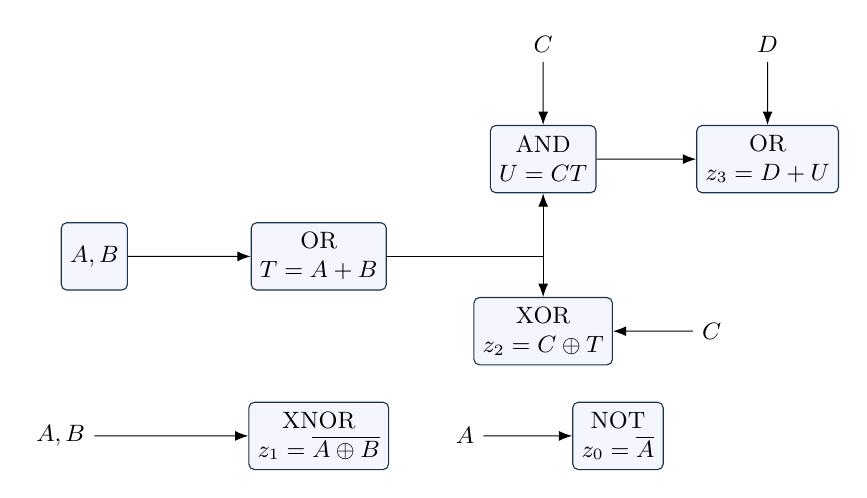
\begin{tikzpicture}[>=Latex,block/.style={draw=ink,rounded corners=2pt,fill=blue!4,minimum height=.9cm,align=center},font=\small,scale=0.95,transform shape]

\node[block] (ab) at (0,2) {$A,B$};\node[block] (t) at (3,2) {OR\\$T=A+B$};
\node[block] (u) at (6,3.3) {AND\\$U=CT$};\node[block] (z3) at (9,3.3) {OR\\$z_3=D+U$};
\node[block] (z2) at (6,1) {XOR\\$z_2=C\oplus T$};
\node[block] (z1) at (3,-.4) {XNOR\\$z_1=\overline{A\oplus B}$};
\node[block] (z0) at (7,-.4) {NOT\\$z_0=\overline A$};
\draw[->] (ab)--(t);\draw[->] (t.east)-|(u.south);\draw[->] (t.east)-|(z2.north);
\draw[->] (u)--(z3);\draw[->] (6,4.6) node[above] {$C$}--(u);
\draw[->] (9,4.6) node[above] {$D$}--(z3);
\draw[->] (8,1) node[right] {$C$} -- (z2.east);
\draw[->] (0,-.4) node[left] {$A,B$}--(z1);
\draw[->] (5.2,-.4) node[left] {$A$}--(z0);

\end{tikzpicture}\end{center}

If an XNOR gate is unavailable, use XOR followed by NOT. This factored network
is multilevel, so its gate cost differs from the independent two-level SOP term count.
\subsection{Prelab question: common anode or common cathode?}
Table 2 represents a \textbf{common-anode display with active-low controls}, as specified
by the handout. For example, digit 0 lights a--f, whose entries are all 0, while g is 1
and stays off. A common-cathode interface normally uses active-high segment signals;
invert the seven outputs if the target interface requires the opposite polarity.

\clearpage\section{Postlab: operating principles and experiment connections}
\subsection{Operating principles, time, and handout issues}
All circuits are combinational. A decoder maps a numeric input to seven segment-control
bits; the ALU produces a numeric result for the selected operation; Gray and excess-3
converters change the representation. After propagation settles, the outputs depend
only on the current inputs. No board clock or register is required. The clocks in the
timing example are simulation stimuli for input enumeration.

Actual total time spent: \underline{\hspace{2cm}} hours.\quad
TA demonstration / sign-off: \underline{\hspace{3cm}}.

Handout issues include the prose/Table 2 conflict for digits 6 and 9, and the unclear
relationship between two \texttt{hex7seg} symbols and the separate letter decoder in
Experiment 3. In Experiment 4, ``a third hex7seg'' should not be read as requiring two
unused instances in that independent project: only two are needed, for HEX2 and HEX3.
\subsection{Global connection rules}
\begin{itemize}
\item This report specifies \textbf{logical board ports}: SW, KEY, LEDR, and HEX.
Physical FPGA \texttt{PIN\_xxx} assignments must come from the course's matching DE0-CV
pin table. Those physical pin numbers have not been checked or invented here.
\item To blank an unused seven-segment display, set all seven outputs to 1. Unused
LEDs may be set to 0. Use explicit logic constants for 0 and 1; do not leave inputs floating.
\item This design inverts each active-low KEY input:
$a_1=\overline{KEY3}$, $a_0=\overline{KEY2}$,
$b_1=\overline{KEY1}$, $b_0=\overline{KEY0}$.
Thus a pressed button represents operand bit 1 and a released button represents 0.
\item Connect by segment index: a to [0], through g to [6]. Do not confuse an
$abcdefg$ pattern with the order of the bus $[6:0]$.
\end{itemize}
\subsection{Experiment 1: displaying a three-bit number}
\noindent\textit{Online circuit illustrations and clickable sources appear in Appendix~\ref{app:webrefs}, with differences from this experiment noted.}

Use the BCD decoder with $D=0$, $C=SW2$, $B=SW1$, and $A=SW0$. Connect outputs a--g
to HEX0[0]--HEX0[6], respectively. Generate each complemented input with NOT gates.


\begin{center}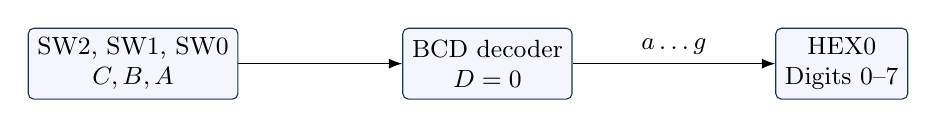
\begin{tikzpicture}[>=Latex,block/.style={draw=ink,rounded corners=2pt,fill=blue!4,minimum height=.9cm,align=center},font=\small,scale=1,transform shape]

\node[block] (sw) at (0,0) {SW2, SW1, SW0\\$C,B,A$};
\node[block] (dec) at (4.5,0) {BCD decoder\\$D=0$};
\node[block] (hex) at (9,0) {HEX0\\Digits 0--7};
\draw[->] (sw)--(dec);\draw[->] (dec)-- node[above] {$a\ldots g$} (hex);

\end{tikzpicture}\end{center}

Set the switches to each value from 000 through 111. Compare the settled display with the expected digit, and record the actual observation separately.

\begin{center}\small
\begin{tabular}{ccccc}
\toprule
SW2 SW1 SW0 & Expected digit & $abcdefg$ & Actual HEX0 & Match?\\\midrule
\texttt{000} & 0 & \texttt{0000001} & \pending & \pending\\
\texttt{001} & 1 & \texttt{1001111} & \pending & \pending\\
\texttt{010} & 2 & \texttt{0010010} & \pending & \pending\\
\texttt{011} & 3 & \texttt{0000110} & \pending & \pending\\
\texttt{100} & 4 & \texttt{1001100} & \pending & \pending\\
\texttt{101} & 5 & \texttt{0100100} & \pending & \pending\\
\texttt{110} & 6 & \texttt{0100000} & \pending & \pending\\
\texttt{111} & 7 & \texttt{0001111} & \pending & \pending\\
\bottomrule\end{tabular}\end{center}


\photo{HEX0 showing a digit, with the corresponding switch positions visible.}

\subsection{Experiment 2: complete hexadecimal display}
\noindent\textit{Online circuit illustrations and clickable sources appear in Appendix~\ref{app:webrefs}, with differences from this experiment noted.}

Replace the BCD decoder with \texttt{hex7seg}. Keep the lower three switch connections
and connect $D$ to SW3. Output a still goes to HEX0[0], through g to HEX0[6]. Verify all
sixteen rows in the target table.


\begin{center}\small
\begin{tabular}{ccccc}
\toprule
SW3--SW0 & Expected glyph & $abcdefg$ & Actual HEX0 & Match?\\\midrule
\texttt{0000} & 0 & \texttt{0000001} & \pending & \pending\\
\texttt{0001} & 1 & \texttt{1001111} & \pending & \pending\\
\texttt{0010} & 2 & \texttt{0010010} & \pending & \pending\\
\texttt{0011} & 3 & \texttt{0000110} & \pending & \pending\\
\texttt{0100} & 4 & \texttt{1001100} & \pending & \pending\\
\texttt{0101} & 5 & \texttt{0100100} & \pending & \pending\\
\texttt{0110} & 6 & \texttt{0100000} & \pending & \pending\\
\texttt{0111} & 7 & \texttt{0001111} & \pending & \pending\\
\texttt{1000} & 8 & \texttt{0000000} & \pending & \pending\\
\texttt{1001} & 9 & \texttt{0000100} & \pending & \pending\\
\texttt{1010} & A & \texttt{0001000} & \pending & \pending\\
\texttt{1011} & b & \texttt{1100000} & \pending & \pending\\
\texttt{1100} & C & \texttt{0110001} & \pending & \pending\\
\texttt{1101} & d & \texttt{1000010} & \pending & \pending\\
\texttt{1110} & E & \texttt{0110000} & \pending & \pending\\
\texttt{1111} & F & \texttt{0111000} & \pending & \pending\\
\bottomrule\end{tabular}\end{center}


\photo{HEX0 displaying one of A, b, C, d, E, or F.}

Experiment 1 LE count: \underline{\hspace{1.5cm}}.\quad
Experiment 2 LE count: \underline{\hspace{1.5cm}}.
Adding hexadecimal constraints reduces minimization freedom; the selected independent
SOPs increase from 15 to 25 terms. Whether the mapped FPGA LE count increases, and by
how much, requires actual compilation reports from the same tool environment.

\clearpage\subsection{Experiment 3: two-bit ALU and two displays}
\noindent\textit{Online circuit illustrations and clickable sources appear in Appendix~\ref{app:webrefs}, with differences from this experiment noted.}

\textbf{Input and output connections.} Invert the four KEY signals as described above.
Connect $S_1=SW1$, $S_0=SW0$. Connect ALU outputs $y_2,y_1,y_0$ to decoder inputs
$C,B,A$, tie $D=0$, and send its segment outputs to HEX0. Send $S_1,S_0$ also to the
letter decoder and connect its seven outputs to HEX1.


\begin{center}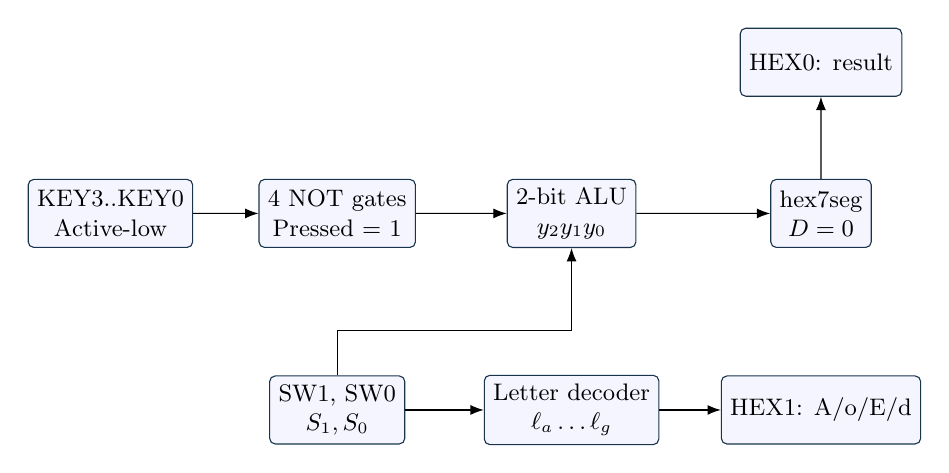
\begin{tikzpicture}[>=Latex,block/.style={draw=ink,rounded corners=2pt,fill=blue!4,minimum height=.9cm,align=center},font=\small,scale=0.96,transform shape]

\node[block] (key) at (0,2) {KEY3..KEY0\\Active-low};
\node[block] (inv) at (3,2) {4 NOT gates\\Pressed = 1};
\node[block] (alu) at (6.1,2) {2-bit ALU\\$y_2y_1y_0$};
\node[block] (dec) at (9.4,2) {hex7seg\\$D=0$};
\node[block] (h0) at (9.4,4) {HEX0: result};
\node[block] (sw) at (3,-.6) {SW1, SW0\\$S_1,S_0$};
\node[block] (ld) at (6.1,-.6) {Letter decoder\\$\ell_a\ldots\ell_g$};
\node[block] (h1) at (9.4,-.6) {HEX1: A/o/E/d};
\draw[->] (key)--(inv);\draw[->] (inv)--(alu);\draw[->] (alu)--(dec);\draw[->] (dec)--(h0);
\draw[->] (sw)--(ld);\draw[->] (ld)--(h1);
\draw[->] (sw.north) -- ++(0,.6) -| (alu.south);

\end{tikzpicture}\end{center}

\textbf{Complete ALU logic.} The following equations allow reconstruction
without an existing Quartus project. First form the two-bit arithmetic sum:
\begin{align*}
t_0&=a_0\oplus b_0,&c_1&=a_0b_0,\\
t_1&=a_1\oplus b_1\oplus c_1,&c_2&=a_1b_1+a_1c_1+b_1c_1.
\end{align*}
For $i=0,1$, use one 4:1 MUX with $I_0=a_ib_i$, $I_1=a_i+b_i$,
$I_2=a_i\oplus b_i$, and $I_3=t_i$. Both MUXs share $S_1,S_0$; their outputs are
$y_i$. The highest result bit is $y_2=S_1S_0c_2$, forcing it to 0 for logic operations.
This implementation is functionally equivalent to the two-slice ALU in Lab 8.

\textbf{Button example.} For arithmetic $3+3=6$, set SW1=SW0=1 and press all four
buttons. After inversion, $a=b=11$ and $y=110$. HEX0 should display 6 and HEX1 should
display d. Since HEX1 is to the left of HEX0, the board reads ``d6'' from left to right.

\clearpage\subsubsection*{Complete theoretical results: all 64 ALU cases}
Each result is $y_2y_1y_0$. The displayed digit is the unsigned value of those three
bits. All entries below are theoretical expectations; the last column is for measurement.


\begin{center}\small
\begin{tabular}{ccccccc}
\toprule
$a_1a_0$ & $b_1b_0$ & AND / A & OR / o & XOR / E & ADD / d & Measured?\\\midrule
\texttt{00} & \texttt{00} & \texttt{000} & \texttt{000} & \texttt{000} & \texttt{000} & \pending\\
\texttt{00} & \texttt{01} & \texttt{000} & \texttt{001} & \texttt{001} & \texttt{001} & \pending\\
\texttt{00} & \texttt{10} & \texttt{000} & \texttt{010} & \texttt{010} & \texttt{010} & \pending\\
\texttt{00} & \texttt{11} & \texttt{000} & \texttt{011} & \texttt{011} & \texttt{011} & \pending\\
\texttt{01} & \texttt{00} & \texttt{000} & \texttt{001} & \texttt{001} & \texttt{001} & \pending\\
\texttt{01} & \texttt{01} & \texttt{001} & \texttt{001} & \texttt{000} & \texttt{010} & \pending\\
\texttt{01} & \texttt{10} & \texttt{000} & \texttt{011} & \texttt{011} & \texttt{011} & \pending\\
\texttt{01} & \texttt{11} & \texttt{001} & \texttt{011} & \texttt{010} & \texttt{100} & \pending\\
\texttt{10} & \texttt{00} & \texttt{000} & \texttt{010} & \texttt{010} & \texttt{010} & \pending\\
\texttt{10} & \texttt{01} & \texttt{000} & \texttt{011} & \texttt{011} & \texttt{011} & \pending\\
\texttt{10} & \texttt{10} & \texttt{010} & \texttt{010} & \texttt{000} & \texttt{100} & \pending\\
\texttt{10} & \texttt{11} & \texttt{010} & \texttt{011} & \texttt{001} & \texttt{101} & \pending\\
\texttt{11} & \texttt{00} & \texttt{000} & \texttt{011} & \texttt{011} & \texttt{011} & \pending\\
\texttt{11} & \texttt{01} & \texttt{001} & \texttt{011} & \texttt{010} & \texttt{100} & \pending\\
\texttt{11} & \texttt{10} & \texttt{010} & \texttt{011} & \texttt{001} & \texttt{101} & \pending\\
\texttt{11} & \texttt{11} & \texttt{011} & \texttt{011} & \texttt{000} & \texttt{110} & \pending\\
\bottomrule\end{tabular}\end{center}


Sixteen operand pairs times four modes give 64 cases. ADD ranges from 0 to 6;
logic results range from 0 to 3. Include carry cases such as $1+3$, $2+2$, $2+3$, and
$3+3$, and confirm $y_2=0$ in each logic mode.

\photo{an ADD result greater than 3 with d beside it, for example HEX1=d and HEX0=6.}

\subsubsection*{Description of the letter decoder}
The design assigns active-low patterns to $00\to A$, $01\to o$, $10\to E$,
$11\to d$, then simplifies each segment function. It uses one XOR, two two-input ANDs,
and two NOTs; a/f share the $S_0$ wire and e/g share constant 0. The same select inputs
drive the ALU and the letters, so the operation label tracks the selected function.
If the second-hex7seg override circuit is used, describe that actual implementation instead.

\clearpage\subsection{Experiment 4: two converters sharing one input}
\noindent\textit{Online circuit illustrations and clickable sources appear in Appendix~\ref{app:webrefs}, with differences from this experiment noted.}

\textbf{Connections:}
\begin{enumerate}
\item Set $b_3=SW3$, $b_2=SW2$, $b_1=SW1$, $b_0=SW0$. Fan out these signals to
the Gray converter, the excess-3 converter, and the input-display decoder.
\item Connect $g_3,g_2,g_1,g_0$ to LEDR3, LEDR2, LEDR1, LEDR0, respectively.
\item Connect $b_3,b_2,b_1,b_0$ to $D,C,B,A$ of one hex7seg; connect its outputs to HEX2.
\item Connect $z_3,z_2,z_1,z_0$ to $D,C,B,A$ of another hex7seg; connect its outputs
to HEX3. Do not tie $z_3$ to 0: unlike Experiment 1, the full four-bit value is required.
\end{enumerate}


\begin{center}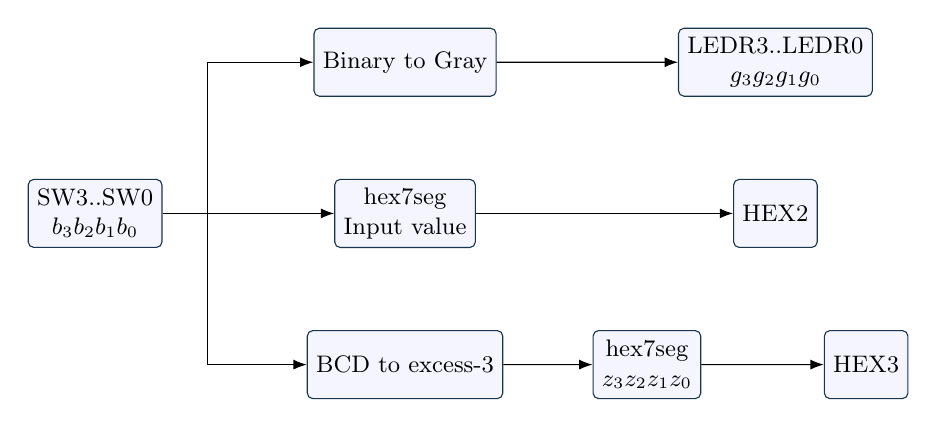
\begin{tikzpicture}[>=Latex,block/.style={draw=ink,rounded corners=2pt,fill=blue!4,minimum height=.9cm,align=center},font=\small,scale=0.96,transform shape]

\node[block] (sw) at (0,0) {SW3..SW0\\$b_3b_2b_1b_0$};
\node[block] (gr) at (4.1,2) {Binary to Gray};
\node[block] (led) at (9,2) {LEDR3..LEDR0\\$g_3g_2g_1g_0$};
\node[block] (inhex) at (4.1,0) {hex7seg\\Input value};
\node[block] (h2) at (9,0) {HEX2};
\node[block] (x3) at (4.1,-2) {BCD to excess-3};
\node[block] (outhex) at (7.3,-2) {hex7seg\\$z_3z_2z_1z_0$};
\node[block] (h3) at (10.2,-2) {HEX3};
\draw[->] (sw.east)--++(.6,0)|-(gr.west);\draw[->] (gr)--(led);
\draw[->] (sw)--(inhex);\draw[->] (inhex)--(h2);
\draw[->] (sw.east)--++(.6,0)|-(x3.west);\draw[->] (x3)--(outhex);\draw[->] (outhex)--(h3);

\end{tikzpicture}\end{center}

\subsubsection*{Gray-code results and the changed bit}
The changed bit compares two consecutive \textbf{settled} Gray outputs. XOR the current
code with the previous code to locate that bit. The first row has no predecessor.


\begin{center}\small
\begin{tabular}{ccccc}
\toprule
$b_3b_2b_1b_0$ & Expected $g_3g_2g_1g_0$ & Changed bit & Actual LEDs & Match?\\\midrule
\texttt{0000} & \texttt{0000} & None (first) & \pending & \pending\\
\texttt{0001} & \texttt{0001} & $g_0$ & \pending & \pending\\
\texttt{0010} & \texttt{0011} & $g_1$ & \pending & \pending\\
\texttt{0011} & \texttt{0010} & $g_0$ & \pending & \pending\\
\texttt{0100} & \texttt{0110} & $g_2$ & \pending & \pending\\
\texttt{0101} & \texttt{0111} & $g_0$ & \pending & \pending\\
\texttt{0110} & \texttt{0101} & $g_1$ & \pending & \pending\\
\texttt{0111} & \texttt{0100} & $g_0$ & \pending & \pending\\
\texttt{1000} & \texttt{1100} & $g_3$ & \pending & \pending\\
\texttt{1001} & \texttt{1101} & $g_0$ & \pending & \pending\\
\texttt{1010} & \texttt{1111} & $g_1$ & \pending & \pending\\
\texttt{1011} & \texttt{1110} & $g_0$ & \pending & \pending\\
\texttt{1100} & \texttt{1010} & $g_2$ & \pending & \pending\\
\texttt{1101} & \texttt{1011} & $g_0$ & \pending & \pending\\
\texttt{1110} & \texttt{1001} & $g_1$ & \pending & \pending\\
\texttt{1111} & \texttt{1000} & $g_0$ & \pending & \pending\\
\bottomrule\end{tabular}\end{center}


\textbf{Transient behavior.} Adjacent target Gray codes differ in one bit,
but this combinational converter is not guaranteed glitch-free during mechanical
switch changes. Changing binary 0111 to 1000 requires four switches and can pass through
other intermediate inputs. Compare outputs only after the intended input has settled.
Synchronous sampling, debouncing, or a direct Gray-sequence generator would be needed
for stronger timing requirements.
\subsubsection*{Excess-3 display results}


\begin{center}\small
\begin{tabular}{cccccc}
\toprule
Input & BCD & Excess-3 & Expected HEX2 & Expected HEX3 & Measured?\\\midrule
0 & \texttt{0000} & \texttt{0011} & 0 & 3 & \pending\\
1 & \texttt{0001} & \texttt{0100} & 1 & 4 & \pending\\
2 & \texttt{0010} & \texttt{0101} & 2 & 5 & \pending\\
3 & \texttt{0011} & \texttt{0110} & 3 & 6 & \pending\\
4 & \texttt{0100} & \texttt{0111} & 4 & 7 & \pending\\
5 & \texttt{0101} & \texttt{1000} & 5 & 8 & \pending\\
6 & \texttt{0110} & \texttt{1001} & 6 & 9 & \pending\\
7 & \texttt{0111} & \texttt{1010} & 7 & A & \pending\\
8 & \texttt{1000} & \texttt{1011} & 8 & b & \pending\\
9 & \texttt{1001} & \texttt{1100} & 9 & C & \pending\\
\bottomrule\end{tabular}\end{center}


For input 5, HEX2 shows 5 and HEX3 shows 8. For inputs 7, 8, and 9, HEX3
shows A, b, and C. It displays the four-bit excess-3 code as a hexadecimal glyph;
it does not expand values 10--12 into two decimal digits. Gray remains defined for
inputs 10--15, but those inputs are invalid BCD and are outside excess-3 acceptance.


\photo{HEX2 showing input 5 and HEX3 showing the corresponding excess-3 value 8.}

\clearpage\section{Postlab: answers to the four questions}
\subsection{Why does the two-bit sum fit one digit? What about a three-bit ALU?}
Unsigned two-bit operands range from 0 to 3, so the maximum sum is $3+3=6=110_2$.
Three binary result bits are needed, but the numeric value is less than 10, so one
decimal seven-segment digit is sufficient.

Unsigned three-bit operands range from 0 to 7, giving a maximum sum of $7+7=14=1110_2$.
The result needs four binary bits. For \textbf{decimal display}, use two digits and
binary-to-decimal/BCD conversion: for $N\in[0,14]$, set the tens digit to
$t=[N\ge10]$ and the units digit to $u=N-10t$, then decode t and u separately.
For \textbf{hexadecimal display}, one existing hex7seg is still sufficient; the maximum
value 14 appears as E. Therefore, two display digits are required for decimal output,
not for every possible output base.
\subsection{Which product term was shared, and how many gates were saved?}
The BCD functions include
\[
a=C\overline A\overline B+A\overline B\overline C\overline D,\qquad
d=C\overline A\overline B+A\overline B\overline C\overline D+ABC.
\]
Sharing the first two terms saves two multi-input AND gates. Sharing $ABC$ between d
and g saves one more, for \textbf{three saved AND gates} under the stated cost model.

For one specific example, $C\overline A\overline B$ is reused by a and d, reducing two
three-input ANDs to one. If only two-input ANDs are allowed, a three-literal product
normally needs two cascaded ANDs, so sharing that product would save two two-input
ANDs instead. State the counting convention. Fan-out buffers are excluded, and these
numbers do not directly determine FPGA LE savings.
\subsection{Why can six extra hexadecimal rows increase decoder cost?}
BCD inputs 10--15 are don't-cares and can be assigned whichever values aid simplification.
Hexadecimal decoding fixes them to letter patterns. Some large groups extending into
the don't-care region become invalid and must be replaced by smaller groups, increasing
terms or literals. The number of \textbf{input constraints} increases even though the
number of outputs stays seven.

Here the selected independently minimized SOPs rise from 15 to 25 total terms. Individual
outputs, alternative glyph choices, or mapped FPGA LE counts need not increase strictly.
For a fixed exact cost model, adding constraints cannot enlarge the feasible implementation
set; the BCD function could already use a full Hex implementation, but its don't-cares
allow a cheaper choice.
\subsection{Why are K-map rows and columns labeled in Gray order?}
The order $00,01,11,10$ makes each adjacent pair differ in exactly one variable, including
the wraparound pair. Thus adjacent minterms can combine using
$XY+X\overline Y=X$, eliminating one variable. Four-cell and eight-cell groups eliminate
two and three variables, respectively.

In ordinary binary order $00,01,10,11$, adjacent labels 01 and 10 differ in two variables.
Treating them as a valid adjacent pair could include unwanted zero minterms, so that
ordering does not support the standard rectangular grouping rule.

\clearpage\section{Verification, conclusions, and remaining evidence}
\subsection{Offline checks actually performed}
The supplied Python generator uses the shared logic engine to generate SOPs with SymPy,
then independently enumerates all cubes and solves an exact covering problem to check
minimum term counts and their minimum literal counts. It evaluates every required
input and compares the ALU gate equations with integer operations.


\begin{center}\small
\begin{tabular}{lc}
\toprule
Check & Passed cases\\\midrule
Valid BCD inputs (all seven segments per input) & 10\\
All Hex inputs (all seven segments per input) & 16\\
Valid excess-3 inputs (all four bits per input) & 10\\
Gray inputs / consecutive settled pairs & 16 / 15\\
ALU cases (result and resulting segment pattern) & 64\\
Letter-select modes, including the override alternative & 4\\
Independent SOP cost checks & 18\\
\bottomrule\end{tabular}\end{center}


The actual results are saved in \texttt{verification.json}. PASS applies to
\textbf{offline Boolean functionality and the specified SOP cost criterion}. It does
not establish FPGA timing, physical pin correctness, LE counts, button debouncing,
or observed display behavior. The theoretical waveform was not run in ModelSim.
\subsection{Design-stage conclusions}
The design derives both BCD and full hexadecimal active-low seven-segment logic.
Don't-cares enable larger K-map groups, while shared product terms reduce duplicated
logic. The letter decoder maps the operation selection to A/o/E/d, and the result
decoder preserves the three-bit ALU result, including the ADD carry. Three adjacent-bit
XORs implement binary-to-Gray conversion; the excess-3 circuit reuses the intermediate
term $A+B$ through factoring.

The main design issues are output polarity, bus bit order, active-low buttons, the
valid BCD domain, decimal versus hexadecimal display, and the distinction between
Gray-code steady-state properties and switching transients. The equations agree with
offline checks. Hardware agreement still requires the listed experiments. This is a
\textbf{design-stage conclusion}, not a claim that the board experiments have been completed.
\subsection{Complete after actual experimentation}
\begin{itemize}
\item Actual problems encountered: \underline{\hspace{8cm}}
\item How they were resolved: \underline{\hspace{8cm}}
\item Measured differences from theory and causes: \underline{\hspace{5cm}}
\item Total time and TA demonstration record: \underline{\hspace{6cm}}
\end{itemize}
\subsection{Submission requirements and current status}


\begin{center}\small
\begin{tabular}{>{\raggedright\arraybackslash}p{4.2cm}>{\raggedright\arraybackslash}p{10.1cm}}
\toprule
Required material & Current status / remaining work\\\midrule
BCD and Hex K-maps & Complete: 14 maps, group elimination, expressions, and shared products.\\
Gray and excess-3 derivations & Complete, including four additional excess-3 K-maps.\\
Schematics and connections & Complete: TikZ diagrams, gate connection tables, and logical board-port mapping.\\
Simulation waveform & Theoretical timing and patterns supplied. A genuine ModelSim screenshot still requires execution.\\
Quartus screenshots and projects & Not created or connected, as requested. These drawings are not Quartus screenshots.\\
Board measurements, photos, and LE counts & Pending actual experiments; all measurement columns are explicitly marked.\\
Postlab questions and conclusions & All four answers and design conclusions are complete. Add actual laboratory experience later.\\
Three project archives and links & Provide actual decoder, ALU-display, and converter projects when available. This document package is not a substitute for those projects.\\
\bottomrule\end{tabular}\end{center}


\appendix
\clearpage\section{Compilation and reproduction without Quartus}
The file \texttt{lab9\_prelab\_postlab.tex} uses TikZ for the design diagrams and a companion images folder for the external reference illustrations. Keep that folder beside the .tex file when compiling. Compile it with XeLaTeX three times to update
the contents and cross-references:
\begin{verbatim}
xelatex -interaction=nonstopmode -halt-on-error lab9_prelab_postlab.tex
xelatex -interaction=nonstopmode -halt-on-error lab9_prelab_postlab.tex
xelatex -interaction=nonstopmode -halt-on-error lab9_prelab_postlab.tex
\end{verbatim}
The English version uses the standard article class and Latin Modern fonts; no Chinese
fonts or ctex package are required. On Overleaf, select XeLaTeX and upload the .tex file together with its images folder.
Common math packages, TikZ, booktabs, fancyhdr, enumitem, and hyperref are required.

Alternatively, run \texttt{build\_pdf.ps1} from the package root in PowerShell.
To regenerate the derivations, checks, CSV, and theoretical VCD, use Python 3.10 or later:
\begin{verbatim}
python -m pip install sympy
python build_lab9.py
\end{verbatim}
Keep \texttt{lab9\_logic.py} beside the English generator: it supplies the shared logic
engine and is imported without generating the Chinese report. Regenerating overwrites
the English .tex file, so back up hand edits first. The VCD contains zero-delay theoretical
values; the CSV contains expected answers, not board observations.

\section{Source files and page references}
\begin{enumerate}
\item \texttt{CPE\_100\_Lab\_9.pdf}: page 2, Table 2 (BCD patterns); page 3,
Table 3 (hexadecimal extension); page 4 (prelab, Gray, and excess-3); pages 5--6
(experiments and connections); page 7 (postlab, grading, and attachments).
\item Adjacent \texttt{lab8/CPE\_100\_Lab\_8.pdf}: page 2, Table 2 (operation codes
00/01/10/11); page 3 (the two-bit ALU and its carry/result outputs).
\end{enumerate}

\clearpage\section{Online circuit illustrations and source links}\label{app:webrefs}
This appendix collects the public circuit references discussed alongside the report.
URLs below each illustration are clickable. Author attribution and scope differences
are retained. These external examples do not establish compilation or board testing
of the designs in this report.
\subsection{Experiments 1 and 2: BCD and full hexadecimal decoders}
The BCD reference supplies a native Quartus BDF file, which requires Quartus to view.
The report's own derivations and connections remain the design for Experiment 1.
The illustration below is Nathan Abel Ortiz's full hexadecimal gate-level decoder,
useful for Experiment 2. It supports 0--F and is not the same minimization as a
BCD-only 0--9 decoder. Check its glyph conventions against this report's target table.
\par\begin{center}
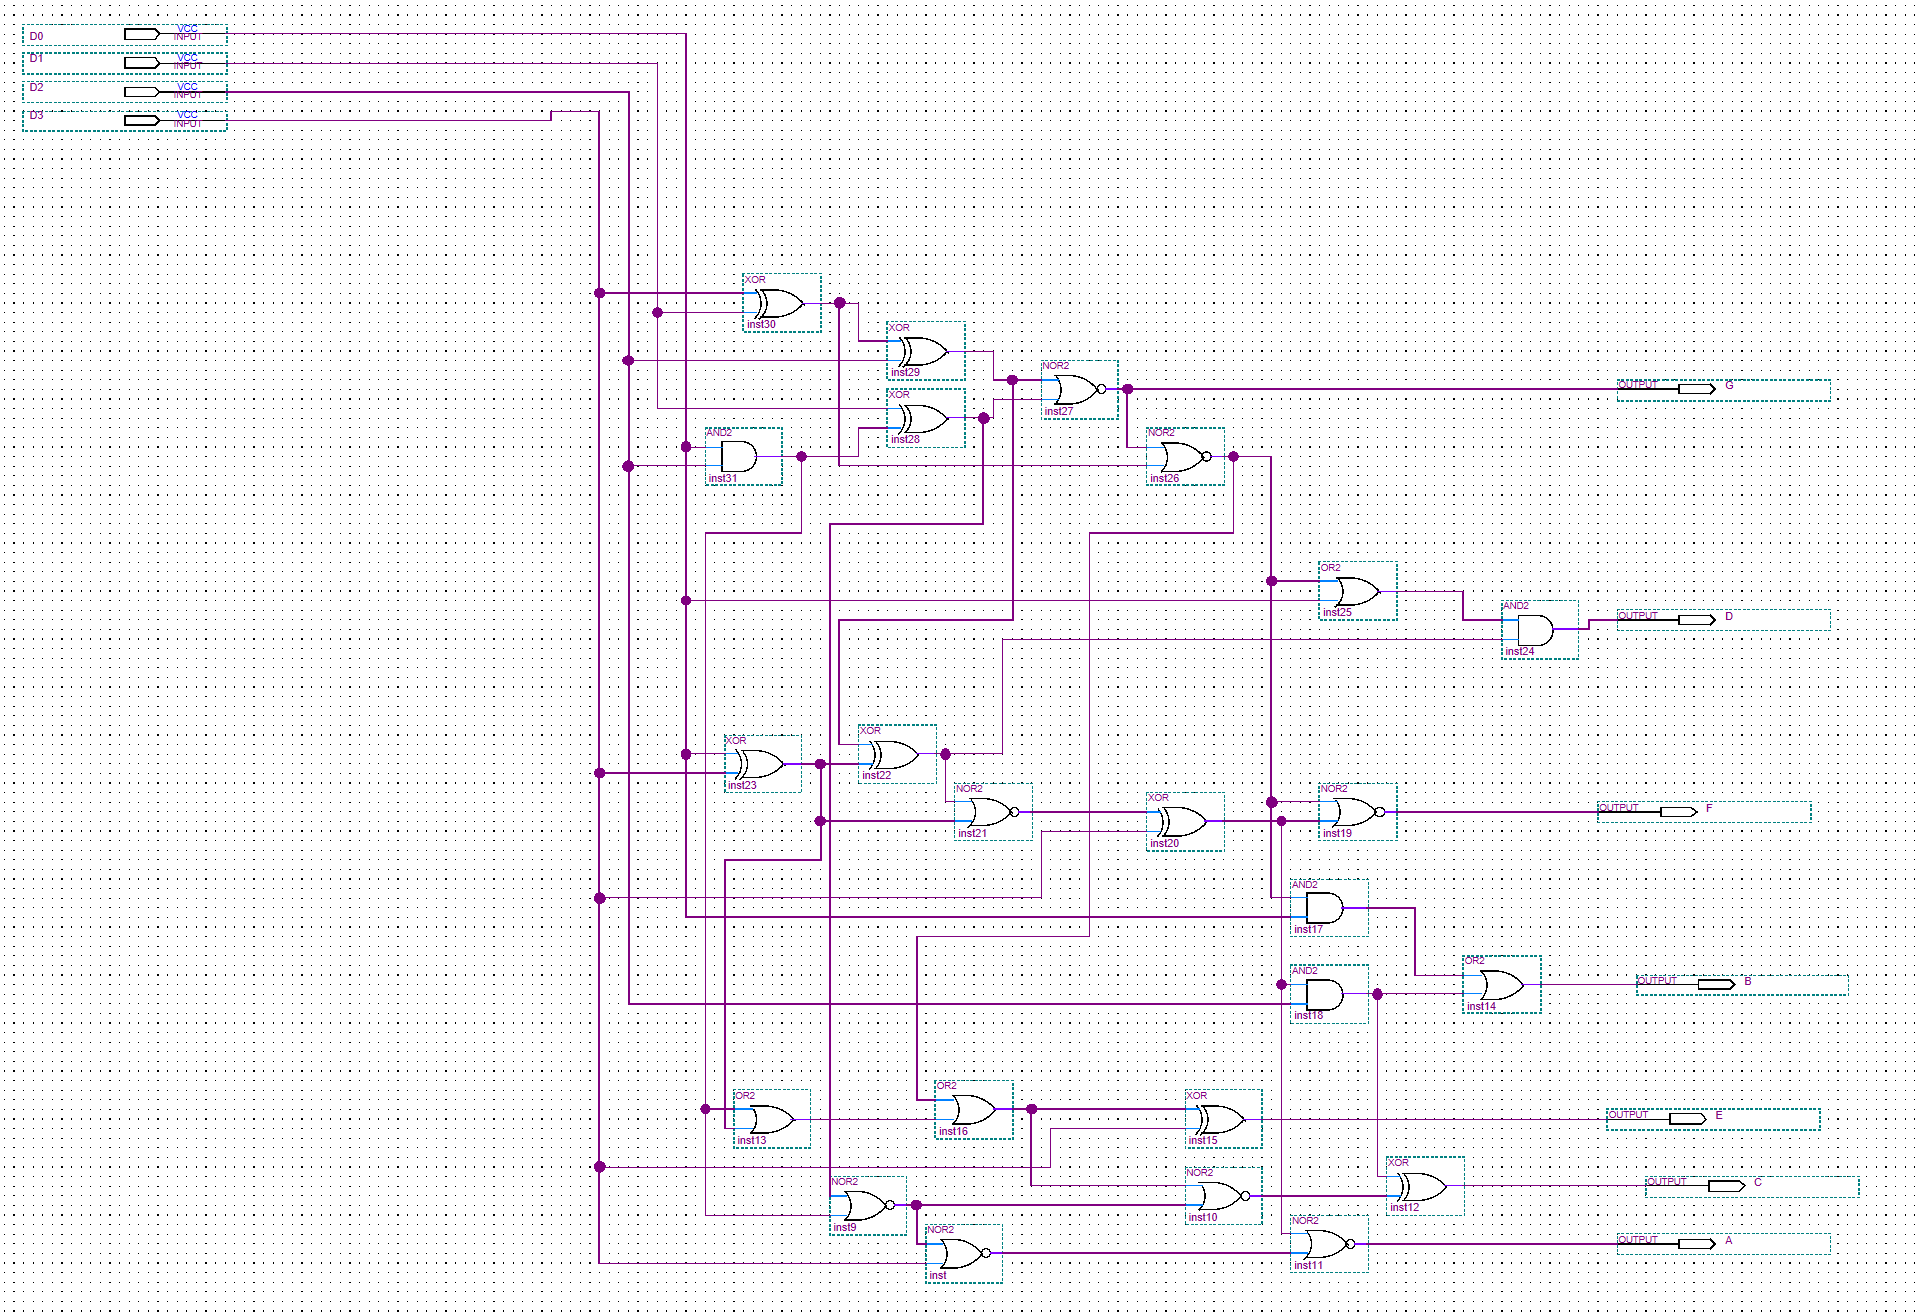
\includegraphics[width=\linewidth,height=.43\textheight,keepaspectratio]{images/hex7-schematic.png}
\par\vspace{.4em}\begin{minipage}{\linewidth}\small\refstepcounter{figure}\figurename~\thefigure: Nathan Abel Ortiz's Quartus hexadecimal seven-segment decoder (external reference).
\end{minipage}\end{center}\par
\par\noindent Experiment 1: native BCD BDF:\par\nopagebreak[4]{\footnotesize\noindent\url{https://github.com/jrmmendes/block-diagram-digital-clock/blob/master/modules/decoders/bcd_to_7segd.bdf}\par}\smallskip

\par\noindent Experiment 2: author project page:\par\nopagebreak[4]{\footnotesize\noindent\url{https://nathanabelortiz.github.io/projects/fpga-hex7.html}\par}\smallskip

\par\noindent Original image:\par\nopagebreak[4]{\footnotesize\noindent\url{https://nathanabelortiz.github.io/assets/projects/fpga/hex7-schematic.png}\par}\smallskip

\clearpage\subsection{Experiment 3: ALU organization and display connections}
The illustration below comes from the University of Jena's Experimental Hardware
Projects course. It shows the operation branches and result selection of a
parameterized ALU. The original diagram illustrates 64 bits; the board exercise
uses four-bit inputs and ADD/SUB/AND/OR. \textbf{Our experiment uses two-bit inputs
and 00 AND, 01 OR, 10 XOR, 11 ADD.} Adapt both the width and control mapping.
\par\begin{center}
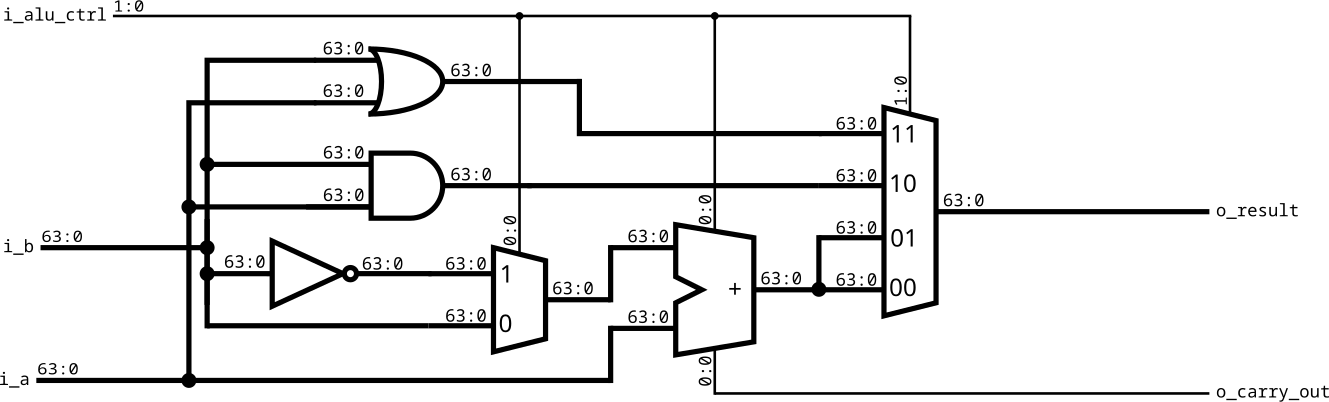
\includegraphics[width=\linewidth,height=.24\textheight,keepaspectratio]{images/alu-basic.png}
\par\vspace{.4em}\begin{minipage}{\linewidth}\small\refstepcounter{figure}\figurename~\thefigure: ALU structure from the University of Jena course (original SVG converted to PNG).
\end{minipage}\end{center}\par
\par\noindent Course page: circuit and display integration:\par\nopagebreak[4]{\footnotesize\noindent\url{https://scalable.uni-jena.de/opt/ehp/chapters/assignment_alu.html}\par}\smallskip

\par\noindent Original SVG:\par\nopagebreak[4]{\footnotesize\noindent\url{https://scalable.uni-jena.de/opt/ehp/_images/alu_basic.svg}\par}\smallskip

\par\noindent Separate four-bit Quartus ALU.bdf example:\par\nopagebreak[4]{\footnotesize\noindent\url{https://github.com/shashwatKanth04/Altera-Quartus-2-Basic-Designs/blob/main/ALU.bdf}\par}\smallskip

The linked BDF contains AND, OR, XOR, arithmetic, and selection blocks and can serve
as a hierarchy reference. Its width and functions still need adaptation. A public
top-level diagram exactly matching our result on HEX0 and A/o/E/d on HEX1 was not
found. Use this report's Experiment 3 dual-display diagram and letter-decoder logic
for those connections.
\clearpage\subsection{Experiment 4: correct four-bit binary-to-Gray circuit}
This diagram is from Thiago Lima's Embarcados tutorial. The most significant bit
passes through; three XOR gates compute the remaining outputs for all 16 inputs.
The article implements the circuit in Verilog. The same gates can be placed
individually in a Quartus BDF schematic.
\par\begin{center}
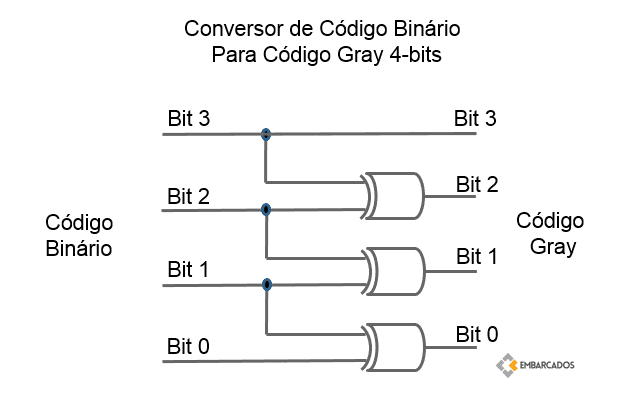
\includegraphics[width=\linewidth,height=.37\textheight,keepaspectratio]{images/gray-4bit.png}
\par\vspace{.4em}\begin{minipage}{\linewidth}\small\refstepcounter{figure}\figurename~\thefigure: Four-bit binary-to-Gray converter: three adjacent-bit XORs and one direct wire. Source: Thiago Lima / Embarcados.
\end{minipage}\end{center}\par
\par\noindent Tutorial and code:\par\nopagebreak[4]{\footnotesize\noindent\url{https://embarcados.com.br/tutorial-de-verilog-codigo-binario-para-codigo-gray/}\par}\smallskip

\par\noindent Original image:\par\nopagebreak[4]{\footnotesize\noindent\url{https://embarcados.com.br/wp-content/uploads/2015/11/gray-7.png}\par}\smallskip

For this experiment, connect SW3--SW0 to the inputs and LEDR3--LEDR0 to the outputs:
\[g_3=b_3,\quad g_2=b_3\oplus b_2,\quad g_1=b_2\oplus b_1,\quad g_0=b_1\oplus b_0.\]
\clearpage\subsection{Experiment 4: BCD-to-excess-3 gate reference}
The hand-drawn diagram below is from Mmamoonn/code-conversion-system. Its lower
half implements excess-3; the upper half shows Gray conversion. This reference
drawing is \textbf{not a Quartus screenshot}.
\par\begin{center}
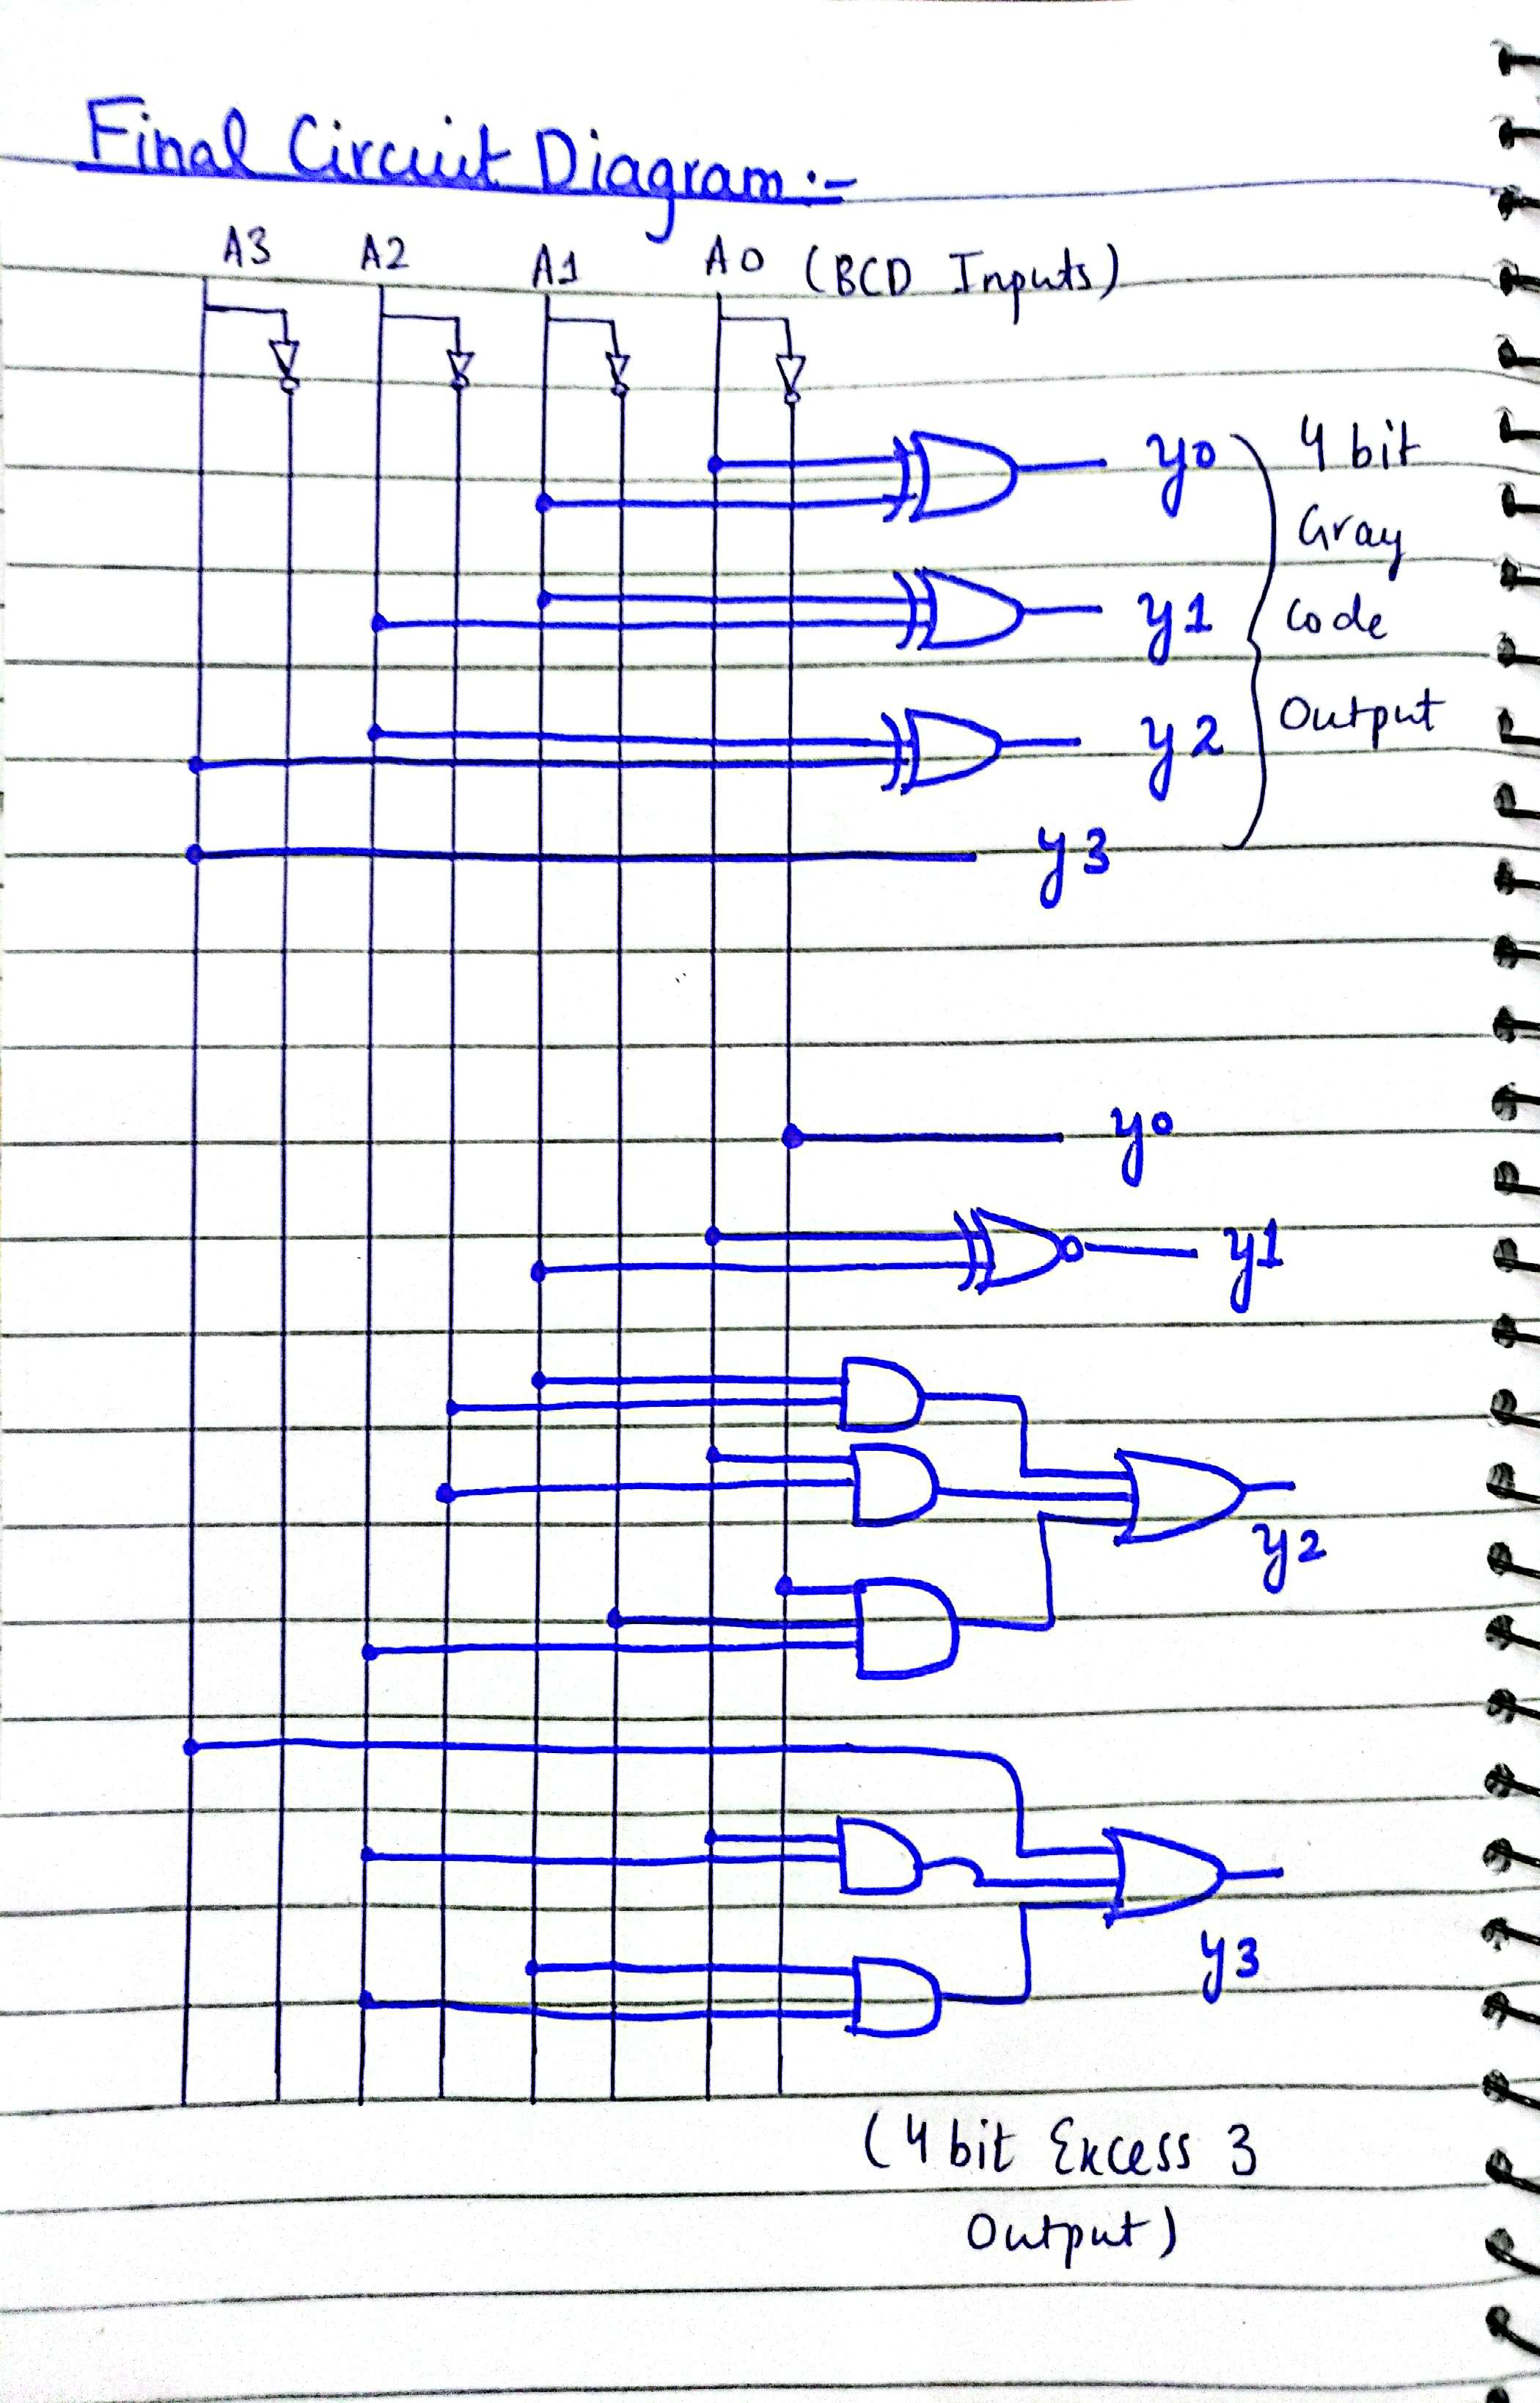
\includegraphics[width=\linewidth,height=.52\textheight,keepaspectratio]{images/converters-combined.jpeg}
\par\vspace{.4em}\begin{minipage}{\linewidth}\small\refstepcounter{figure}\figurename~\thefigure: Combined Gray and excess-3 reference drawing. Source: GitHub user Mmamoonn. The lower half is the excess-3 circuit.
\end{minipage}\end{center}\par
\par\noindent Circuit drawing source:\par\nopagebreak[4]{\footnotesize\noindent\url{https://github.com/Mmamoonn/code-conversion-system/blob/main/hardware/circuit-diagrams/final_circuit_diagram.jpeg}\par}\smallskip

\par\noindent Structural excess-3 VHDL:\par\nopagebreak[4]{\footnotesize\noindent\url{https://github.com/Mmamoonn/code-conversion-system/blob/main/vhdl/src/bcdtoex3.vhd}\par}\smallskip

\par\noindent Gray source requiring care:\par\nopagebreak[4]{\footnotesize\noindent\url{https://github.com/Mmamoonn/code-conversion-system/blob/main/vhdl/src/bcdtogray.vhd}\par}\smallskip

\textbf{Drawing/code discrepancy:} the repository's Gray code uses OR for $g_2$,
whereas the drawing shows XOR. OR agrees with this XOR on valid BCD inputs 0--9
but fails for binary inputs 12--15. Use the preceding three-XOR circuit for our
0--15 Gray tests. Excess-3 tests cover valid BCD inputs 0--9: display the input
through a BCD decoder on HEX2 and the converted code through a Hex decoder on HEX3.

\end{document}
